\documentclass[10pt]{article}

\usepackage{blindtext}
\usepackage{etex}
\usepackage{makeidx}  % allows for indexgeneration
\usepackage{mathtools} %
\usepackage{booktabs} %
\usepackage{verbatim} %
\usepackage{graphicx} 
\usepackage{amsmath}
\usepackage{amssymb}
\usepackage{amsthm}
\usepackage{xspace}
\usepackage{natbib}
\usepackage{pifont}%
\usepackage{tikz}
\usepackage{relsize}
\usepackage{multirow}
\usepackage{textcomp}
\usepackage{comment}
\usepackage{url}
\usepackage{float}
\usepackage{algorithm}
\usepackage{algpseudocode}
\usepackage{subfig}
\usepackage{framed}
\usepackage{empheq}

\newcommand{\cmark}{\ding{51}}%
\newcommand{\xmark}{\ding{55}}%
\newcommand{\vectornorm}[1]{\left|\left|#1\right|\right|}
\newcommand{\argmin}{\operatornamewithlimits{argmin}}
\newcommand{\argmax}{\operatornamewithlimits{argmax}}

\algdef{SE}[DOWHILE]{Do}{doWhile}{\algorithmicdo}[1]{\algorithmicwhile\ #1}%

\newtheorem{problem}{Problem}

\newcommand{\Tempselect}{\textit{TempSelect}\xspace}

%\excludecomment{plots}
%\includecomment{plots}

\begin{document}

\title{Efficient Selection of Optimal Time Points Over Biological Time-Series Data}
\date{}

\maketitle


\section{Supplementary Results}


\subsection{\Tempselect Pseudocode}

Pseudocode of \Tempselect is in Algorithm~\ref{alg:algo}.

\begin{algorithm}
\caption{\Tempselect: Iterative $k$-point selection}
\label{alg:algo}
\begin{algorithmic}[1]
\Procedure{Iterative\textendash Temporal\textendash Selection}{}
\State $C_{0} = $ select initial $k$ time points by absolute difference sorting
\State $e_{0} = $ error of remaining points by fitting splines to $C_{0}$
\State $i=0$
\Do 
\For{each pair $(t_{a}, t_{b}) \in (T^{-} \setminus C_{i}) \times C_{i}$}
\State $C^{*} = C_{i} \cup \{ t_{a} \} \setminus \{ t_{b}\}$ 
\State $e^{*} = $ estimate error by fitting smoothing spline to
$C^{*}$ where \par 
\hspace{1.62cm} regularization parameter is estimated by LOOCV
\If{$e^{*} < e_{i}$}
\State $C_{i+1} = C^{*}$ 
\State $e_{i+1} = e^{*}$
\EndIf
\State $i = i+1$
\EndFor
\doWhile{$e_{i+1} < e_{i}$}
\State Output $C_{i}$ and $e_{i}$
\EndProcedure
\end{algorithmic}
\end{algorithm}


\subsection{miRNA Clusters Are Enriched For Several Biological Processes}\label{sec:mirna}

Detailed analysis of miRNA dataset shows clustered expression profiles
of miRNAs as in Figure~\ref{fig:clustmirna}. We identified $8$ stable miRNA
clusters by k-means algorithm~\cite{kmeans} where the number of clusters is selected by
Bayesian Information Criteria~\cite{bic}. We find clusters to change more frequently
than mRNA data as miRNA is noisier than mRNA data which clusters are in Figure~\ref{fig:supclust}. After mapping each miRNA to
the set of corresponding genes by TargetScan~\cite{agarwal2015}, we run
gene-enrichment analysis by FuncAssociate~\cite{berriz2003}. We find clusters to be enriched
for several Gene Ontology biological processes~\cite{go}. For
instance, cluster $4$ is enriched for single-organism cellular
process, positive regulation of biological process, regulation of
metabolic process, etc.

\begin{figure}
\centering
\includegraphics[scale=0.25]{{plots/mirnadata/centplot}.png}
\caption{$8$ stable clusters}
\label{fig:clustmirna}
\end{figure}

\begin{figure}
\begin{minipage}{1.0\textwidth}
\subfloat[6 stable clusters]{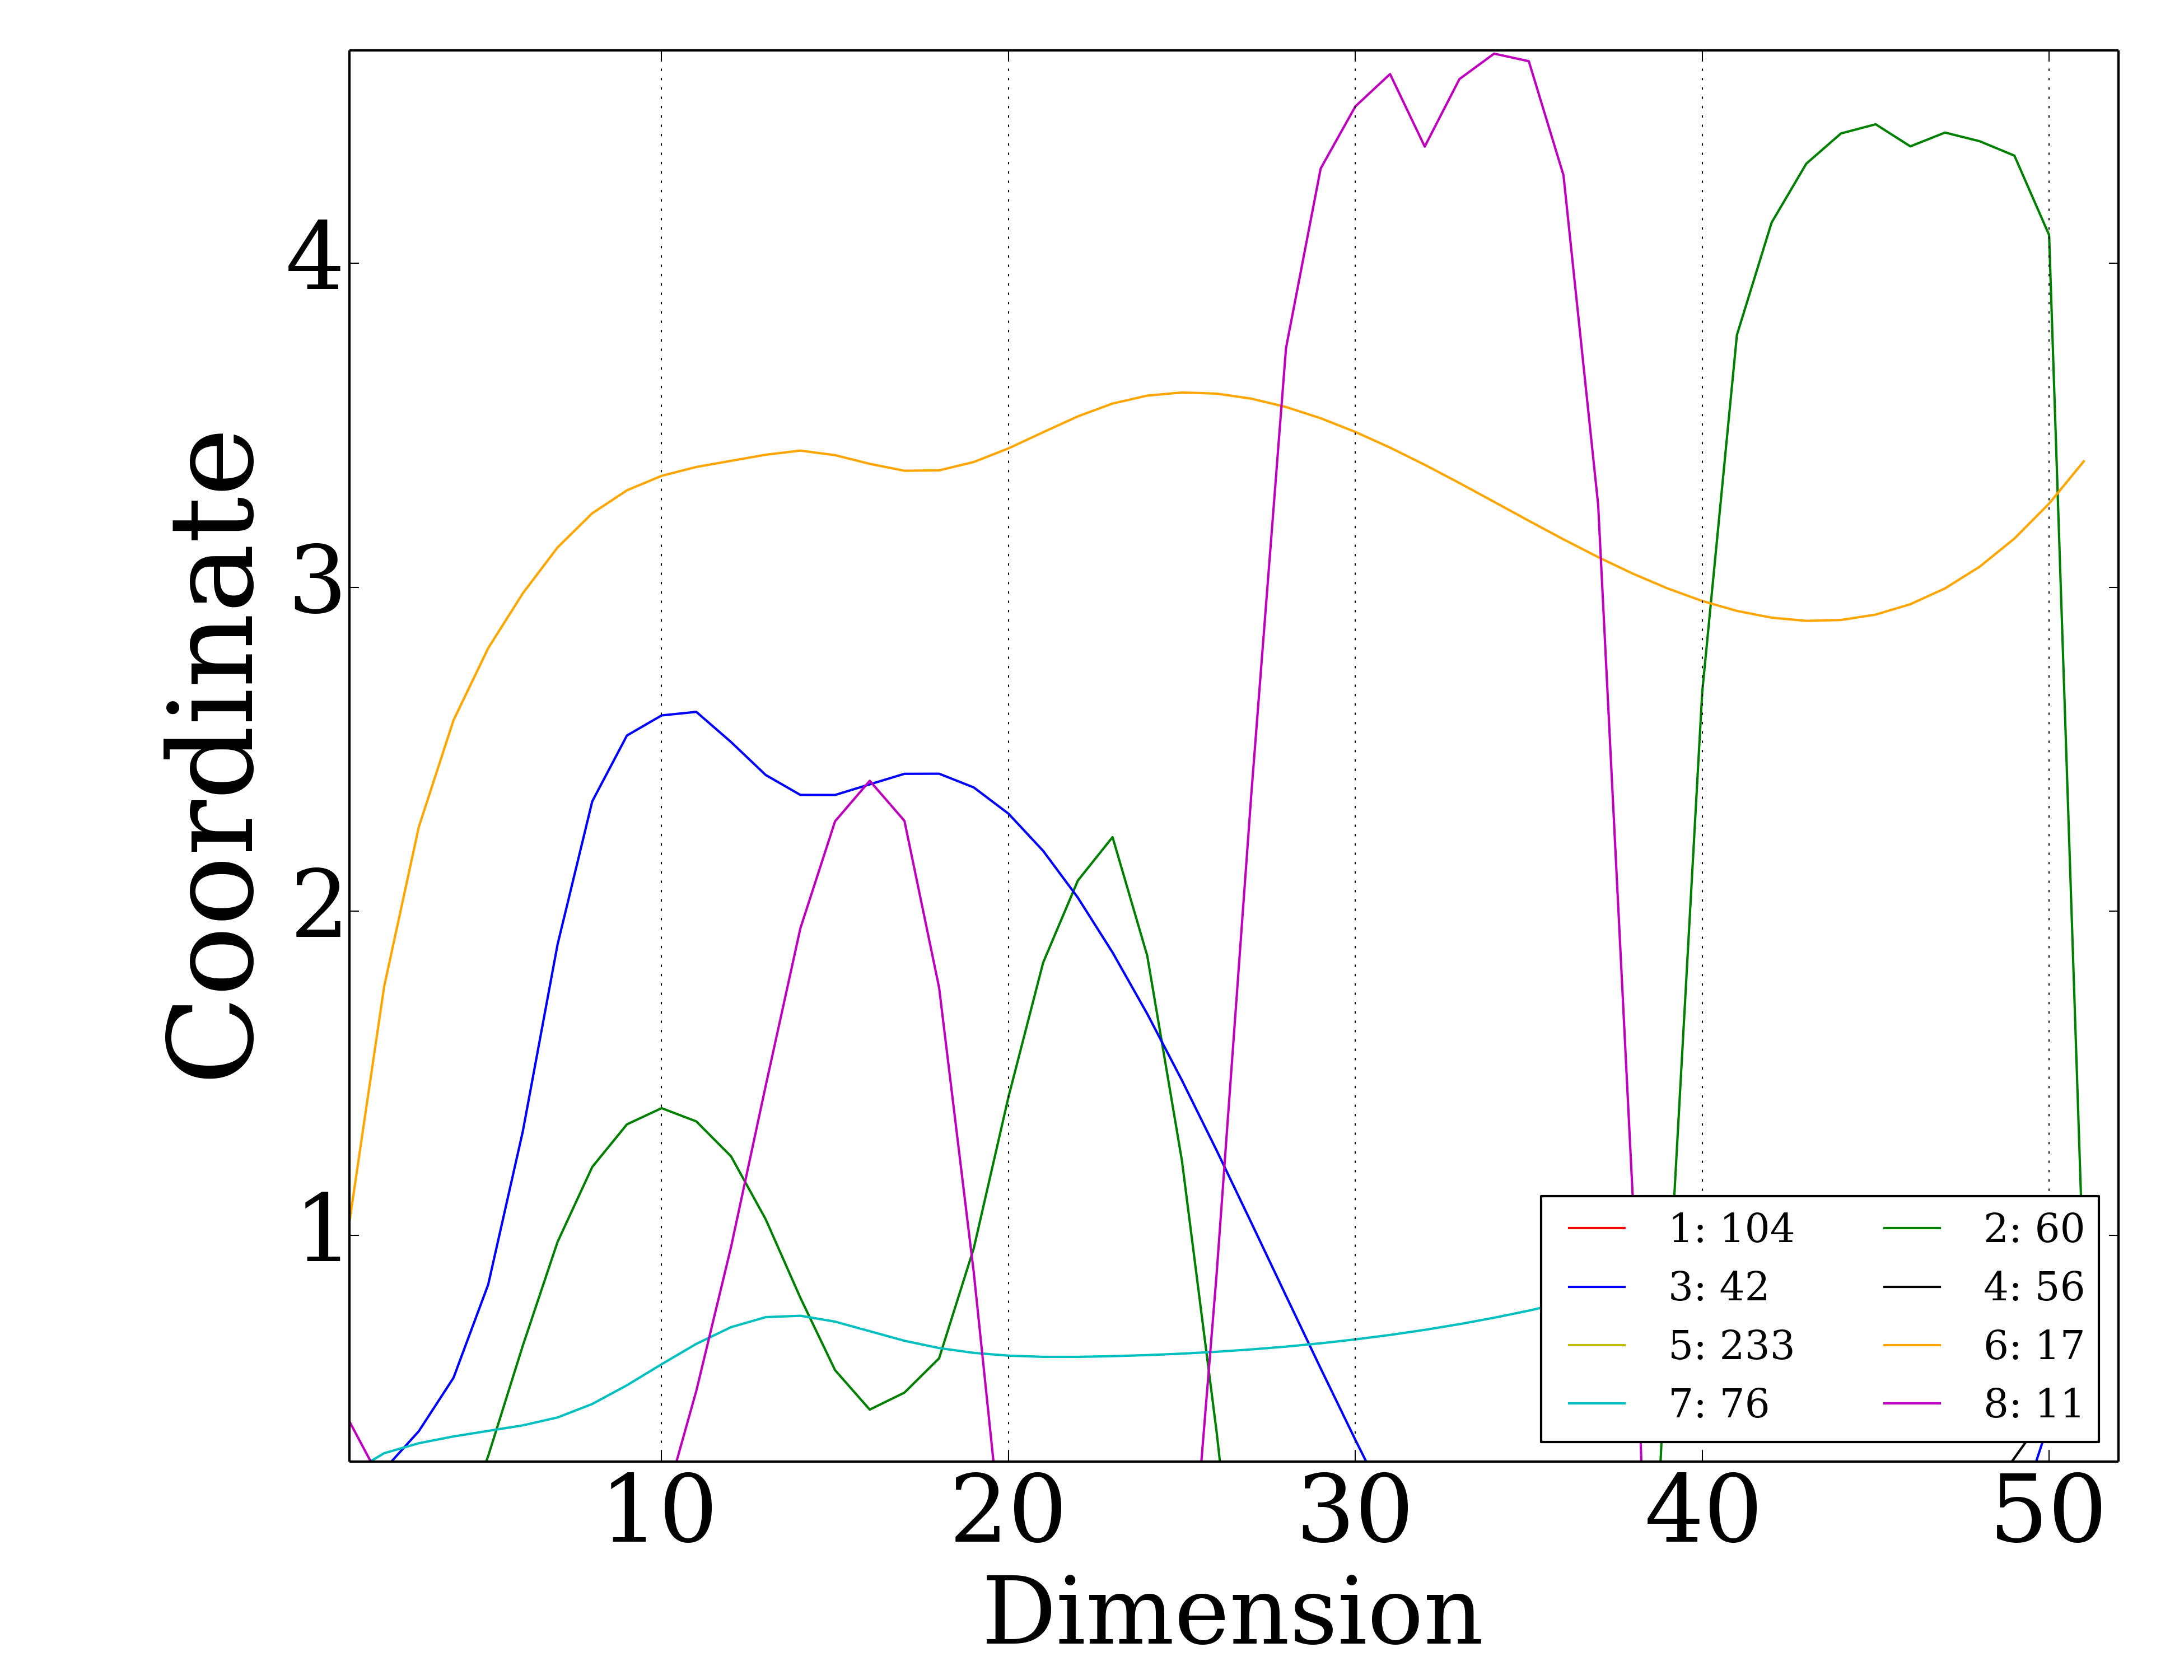
\includegraphics[scale=0.2]{{plots/newdata/centplotlimit}.png}}
\hfill
\subfloat[Centroids]{\includegraphics[scale=0.2]{{plots/newdata/centplot}.png}}
\end{minipage}
\caption{}
\label{fig:supclust}
\end{figure}


\subsection{Selecting time points for Methylation analysis}\label{sec:compareboth}

% \Tempselect identified $0.5$, $5$, $15$, $26$ as candidate points out
% of $8$ time points over temporal methylation data when we consider
% each locus independently. When we only use the same $8$ time points over
% gene-expression dataset, we also identified $0.5$, $5$, $15$, $26$ by running
% \Tempselect over all subset of possible time points. We have also
% found either high positive or high negative correlation between both
% datasets by plotting them jointly as in Figure~\ref{fig:methgene} for
% DNMT3A, SRC, and LOX genes. Among the multiple methylation loci belonging to a gene, we select
% the most correlated one in terms of absolute value of pearson correlation~(See
% Supplementary Table~\ref{tab:sup2} for correlation of all genes and
% Supplementary Fig.~\ref{fig:sup7} for distribution of correlation for loci of each gene). Overall,
% similarity of the identified points when combined with the similarity
% of the curves in the Figure suggest the possibility of global set of
% time points that are important for both genomic and epigenetic
% experiments. 

\section{Supplementary Figures}

%\tableofcontents
%\addcontentsline{toc}{section}{\listfigurename}
%\listoffigures
%\addcontentsline{toc}{section}{\listtablename}
%\listoftables

%extra supporting
% We find that best informed guess is to initialize using points that are sorted by increasing absolute
% differences. Using additional anchor points such as E16.5 and E18.5
% for analyses leads to similar results. We also enumerated top $10$ optimal solutions by running \Tempselect
% across many initial conditions. We find selected points and errors of
% these solutions to be quite similar to our solution above~(See
% Supplementary Table~\ref{tab:xxx}). This trend is also observed when
% we select fewer points, we find similar results when we enumerate all
% possible solutions of size $6$ to examine the optimality structure of the solution space. 

\subsection{\Tempselect identifies subset of important time points across multiple genes}

To understand whether gene-expression profiles over time has a simple
trend, we also compare the reconstruction performance of \Tempselect
with fitting piecewise linear curves between initial and middle time points
and between middle and last time points. The reconstruction error by
\Tempselect is significantly better than the piecewise linear reconstruction for $102$ genes out of $126$ genes. We have plotted the
comparison of reconstruction for several of these genes as in Supplementary Figure~\ref{fig:sup5}. The distribution of error difference between
these methods looks significantly different than normal distribution~($p < 0.0001$ by Shapiro-Wilk test).

\setcounter{figure}{0}   
\begin{figure}[ht]
\centering
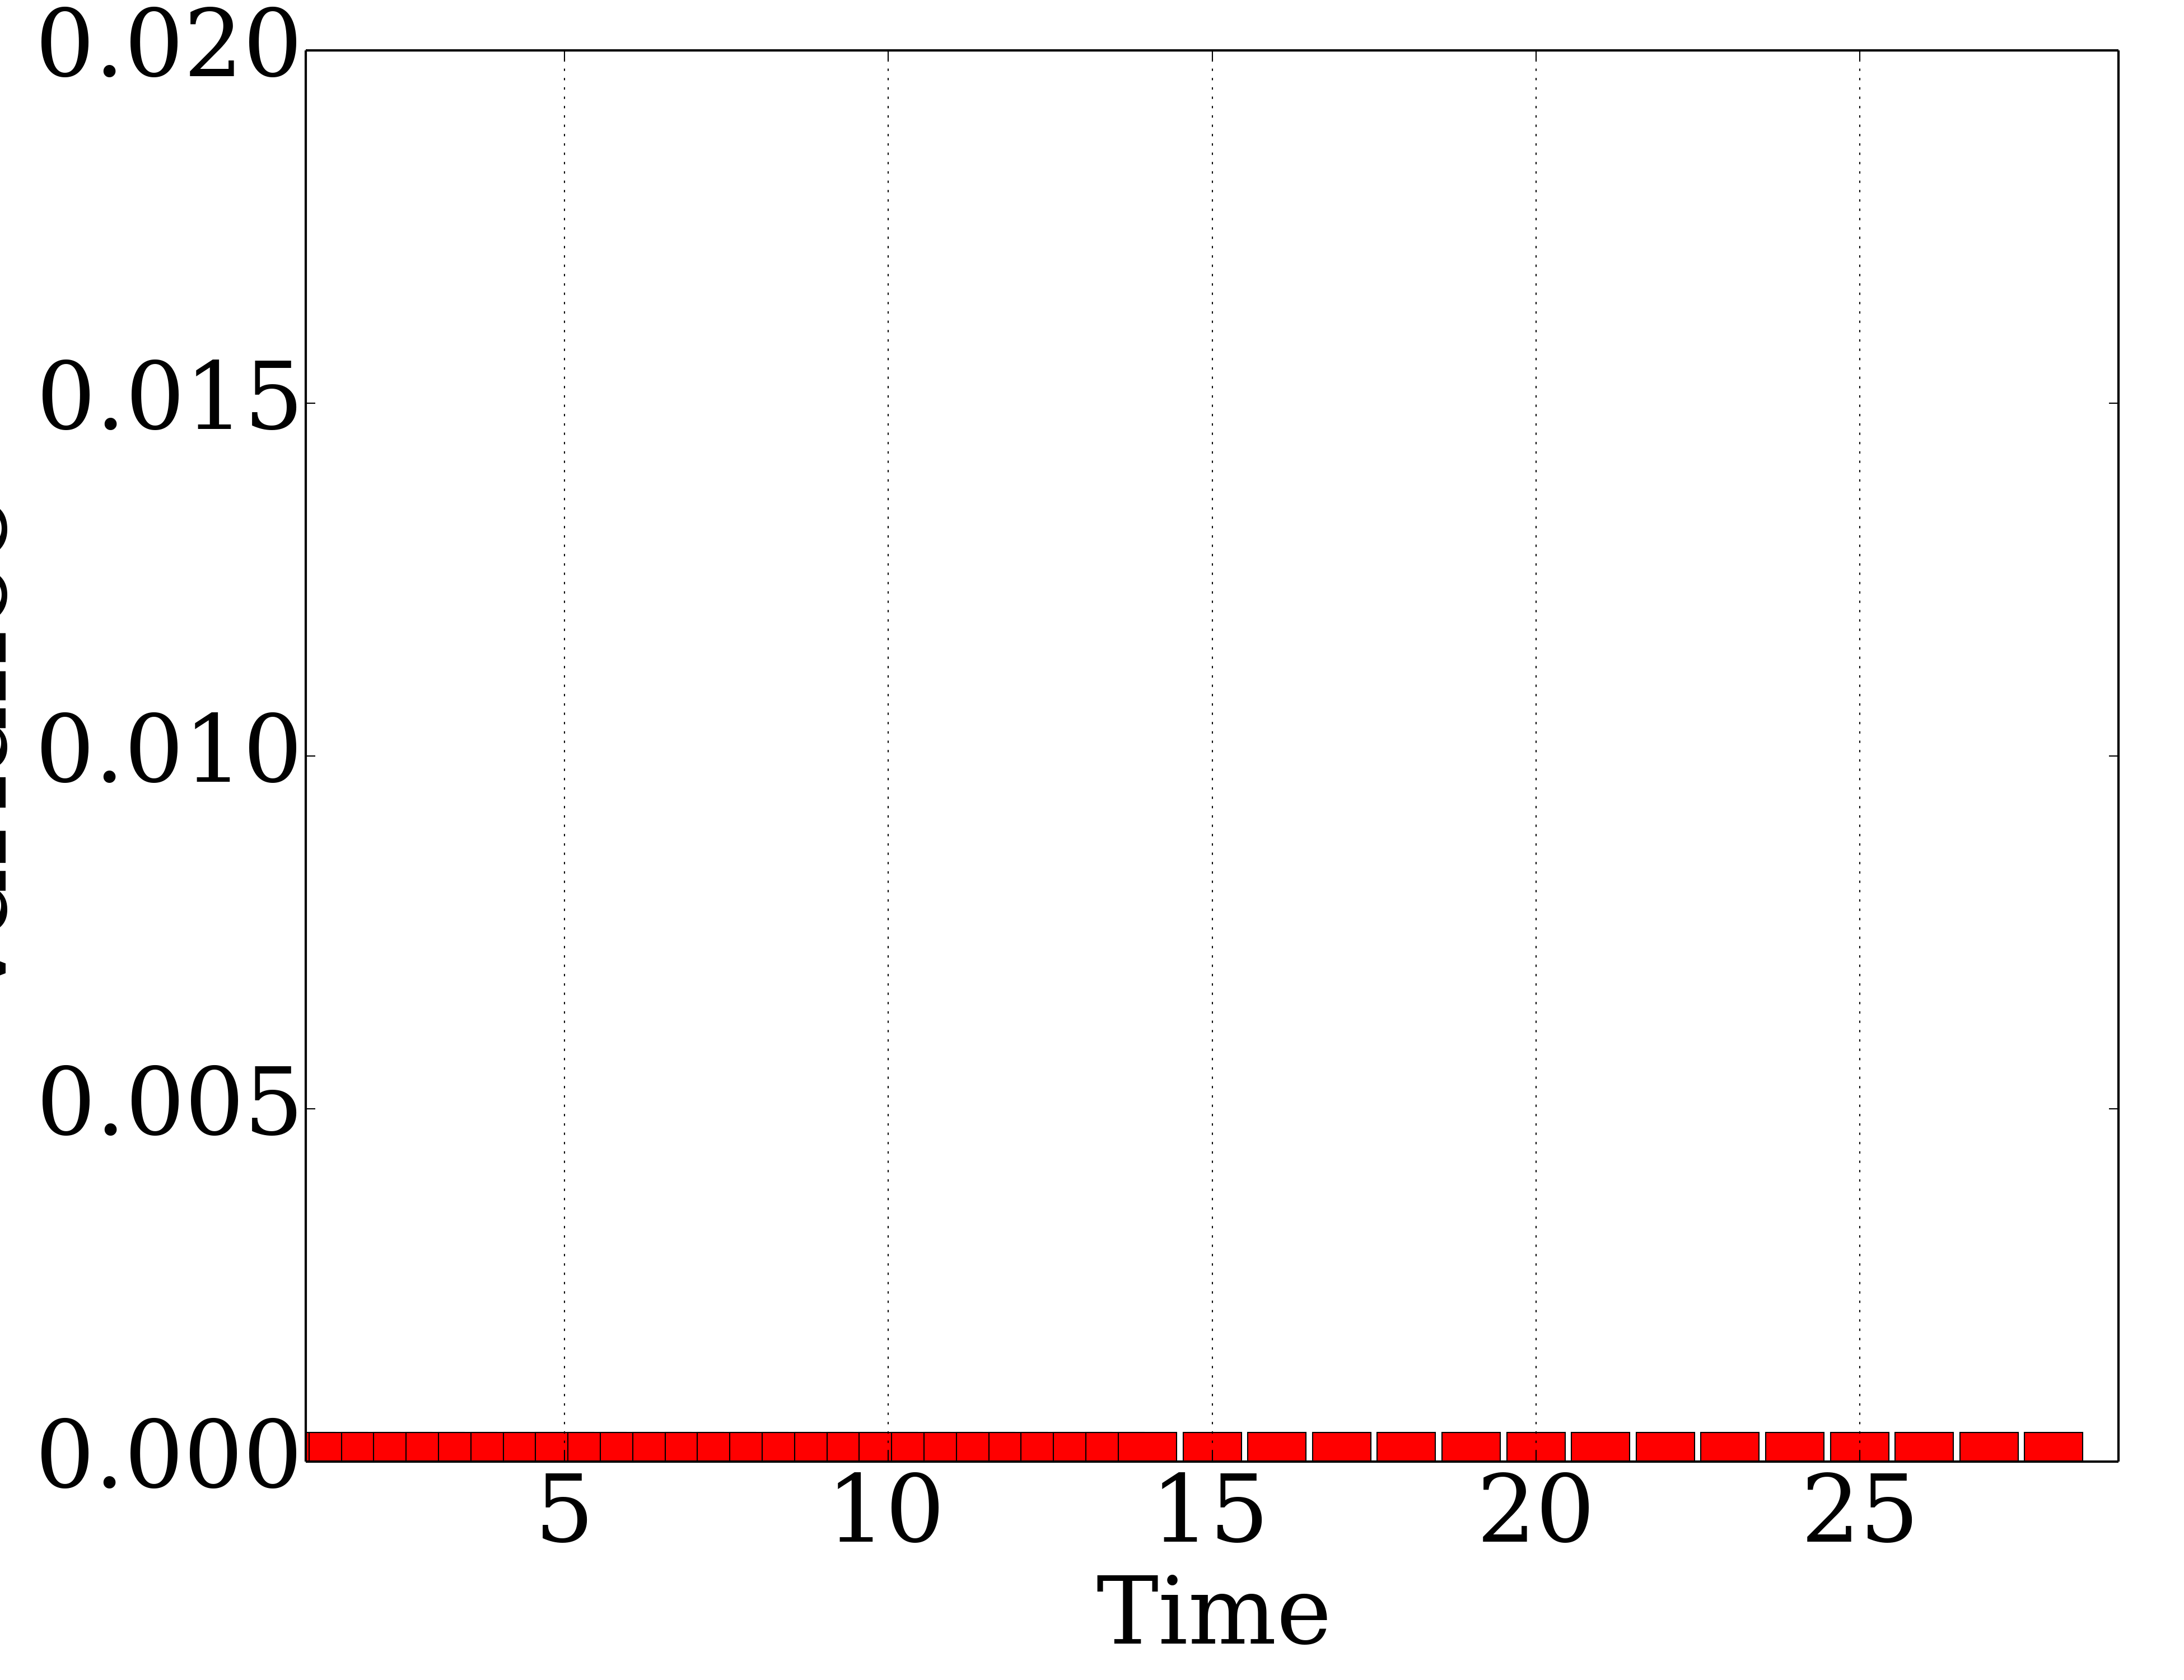
\includegraphics[scale=0.25]{{plots/newdata/timeerror}.png}
\caption{Average noise in each time point}
\label{fig:sup1}
\end{figure}

\begin{figure}
\centering
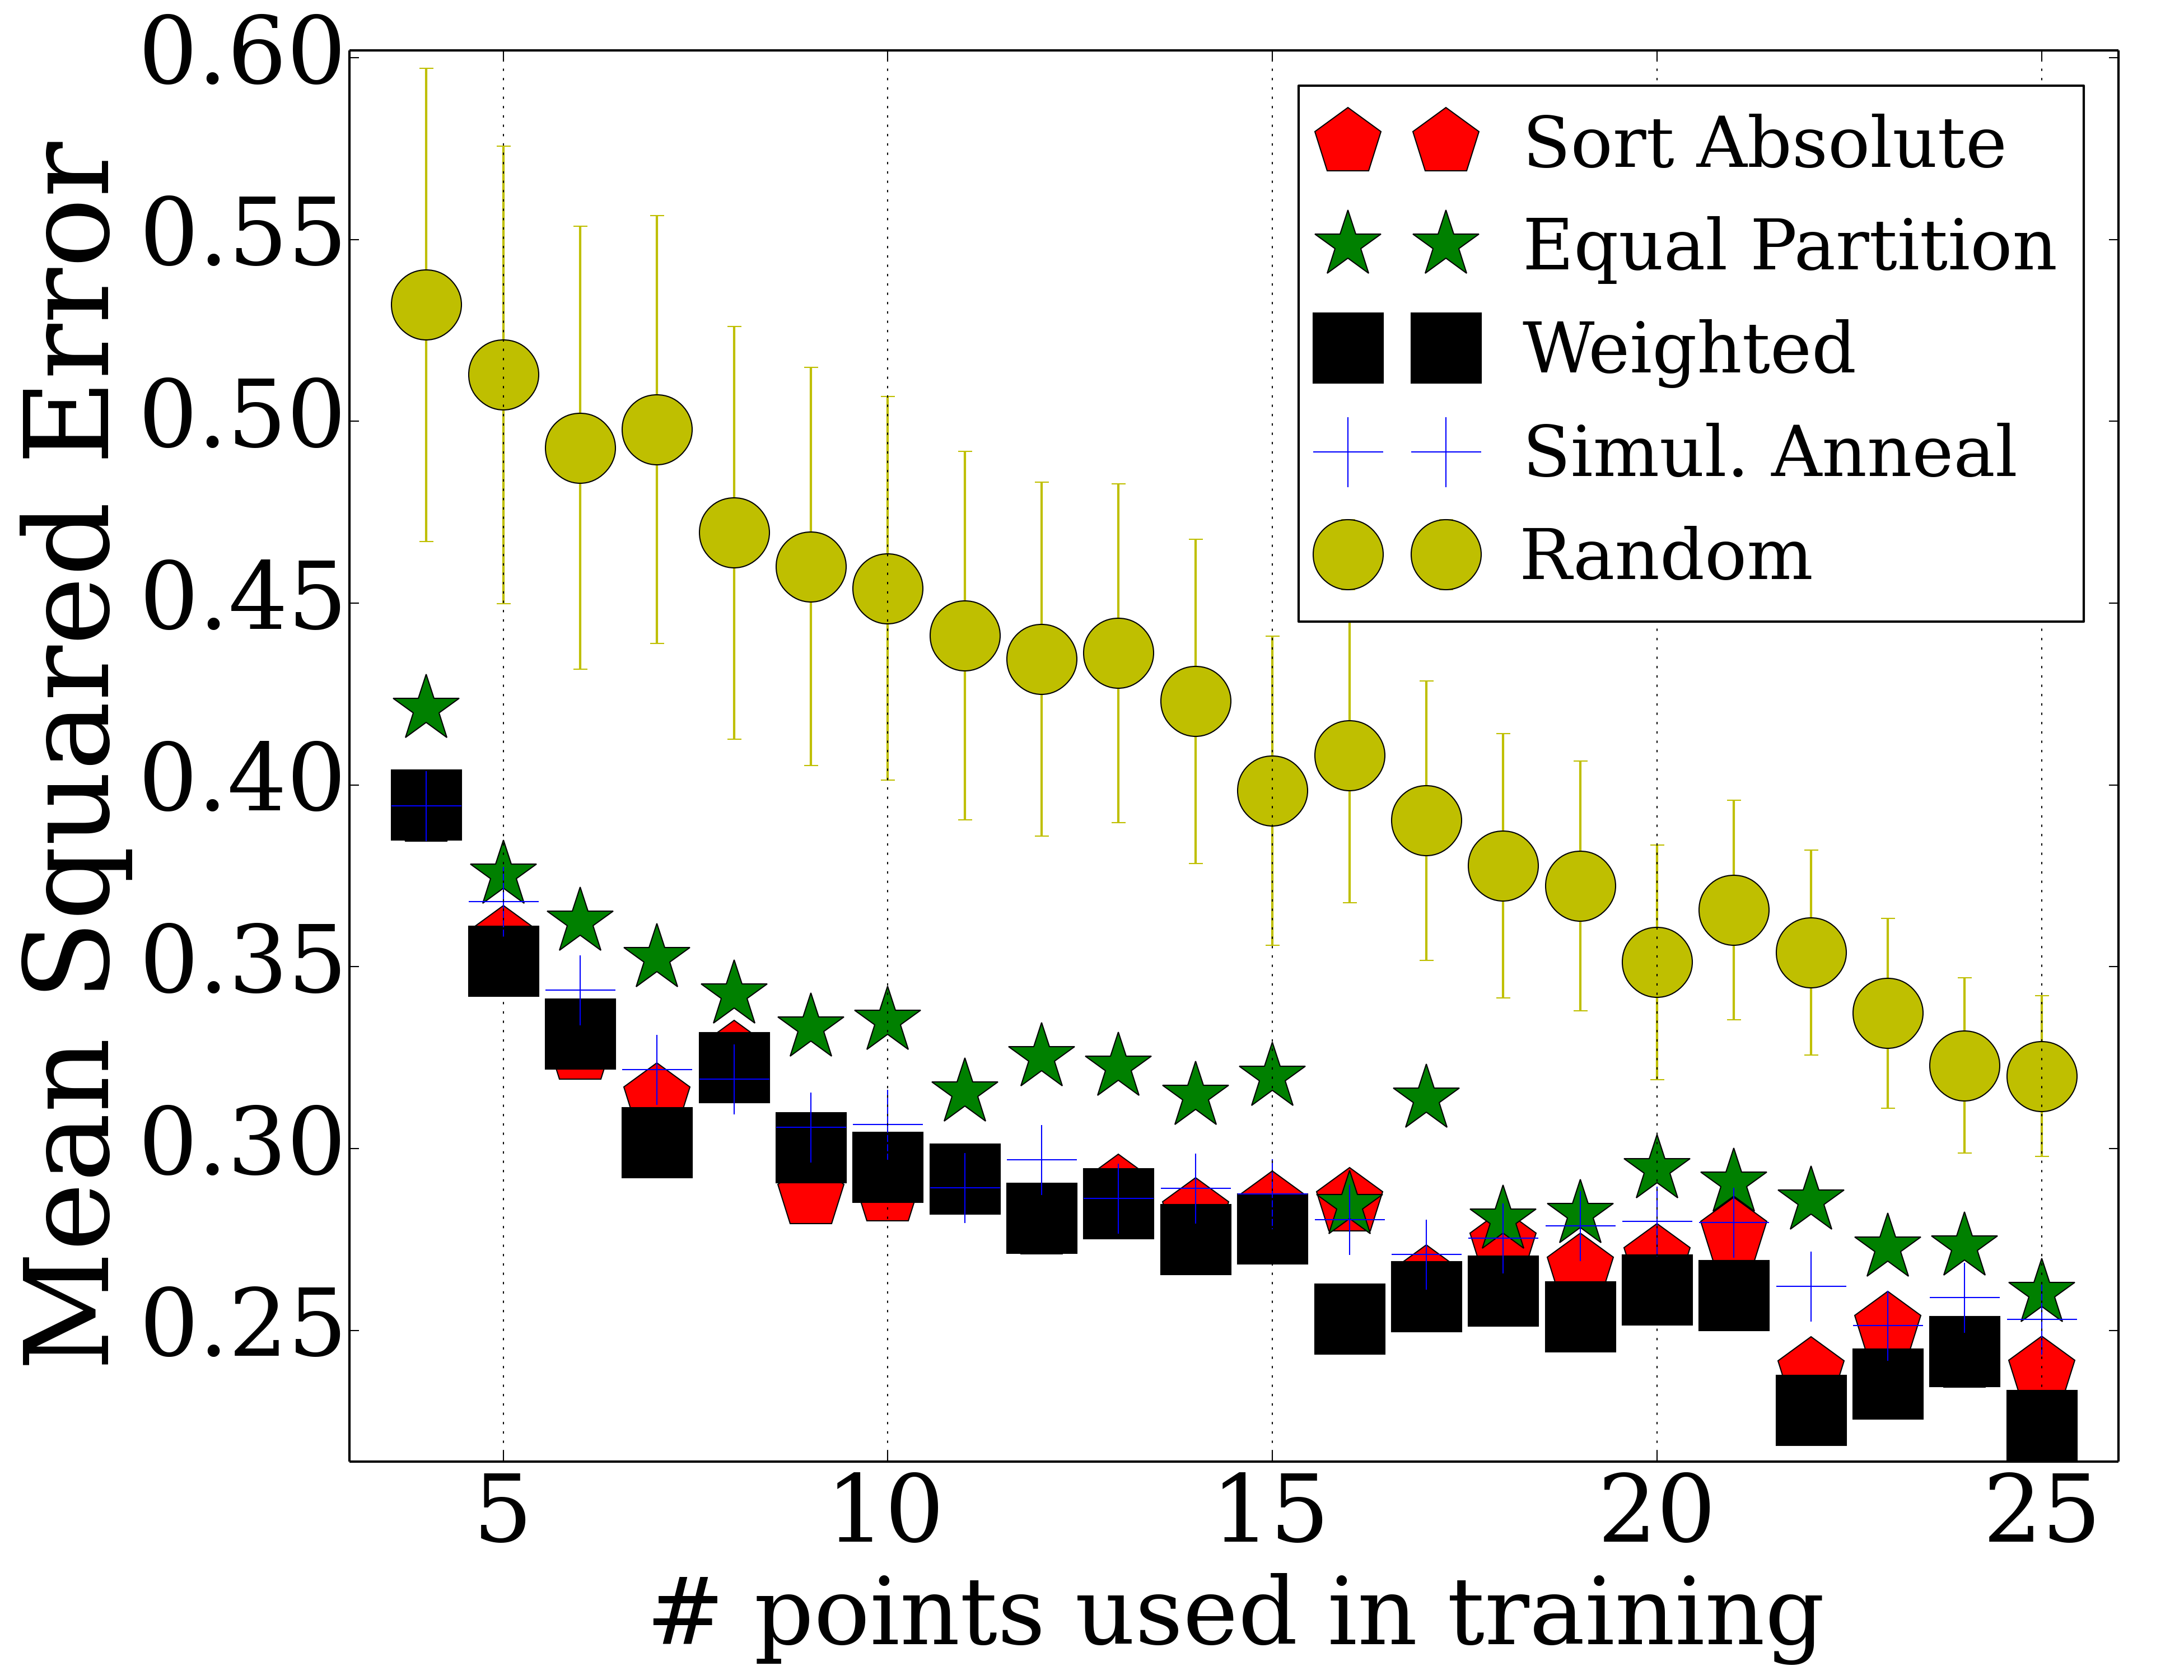
\includegraphics[scale=0.25]{{plots/newdata/performRL2}.png}
\caption{Performance of \Tempselect by increasing number of selected points}
\label{fig:sup2}
\end{figure}

\begin{figure}
\begin{minipage}{1.0\textwidth}
\subfloat[ERB]{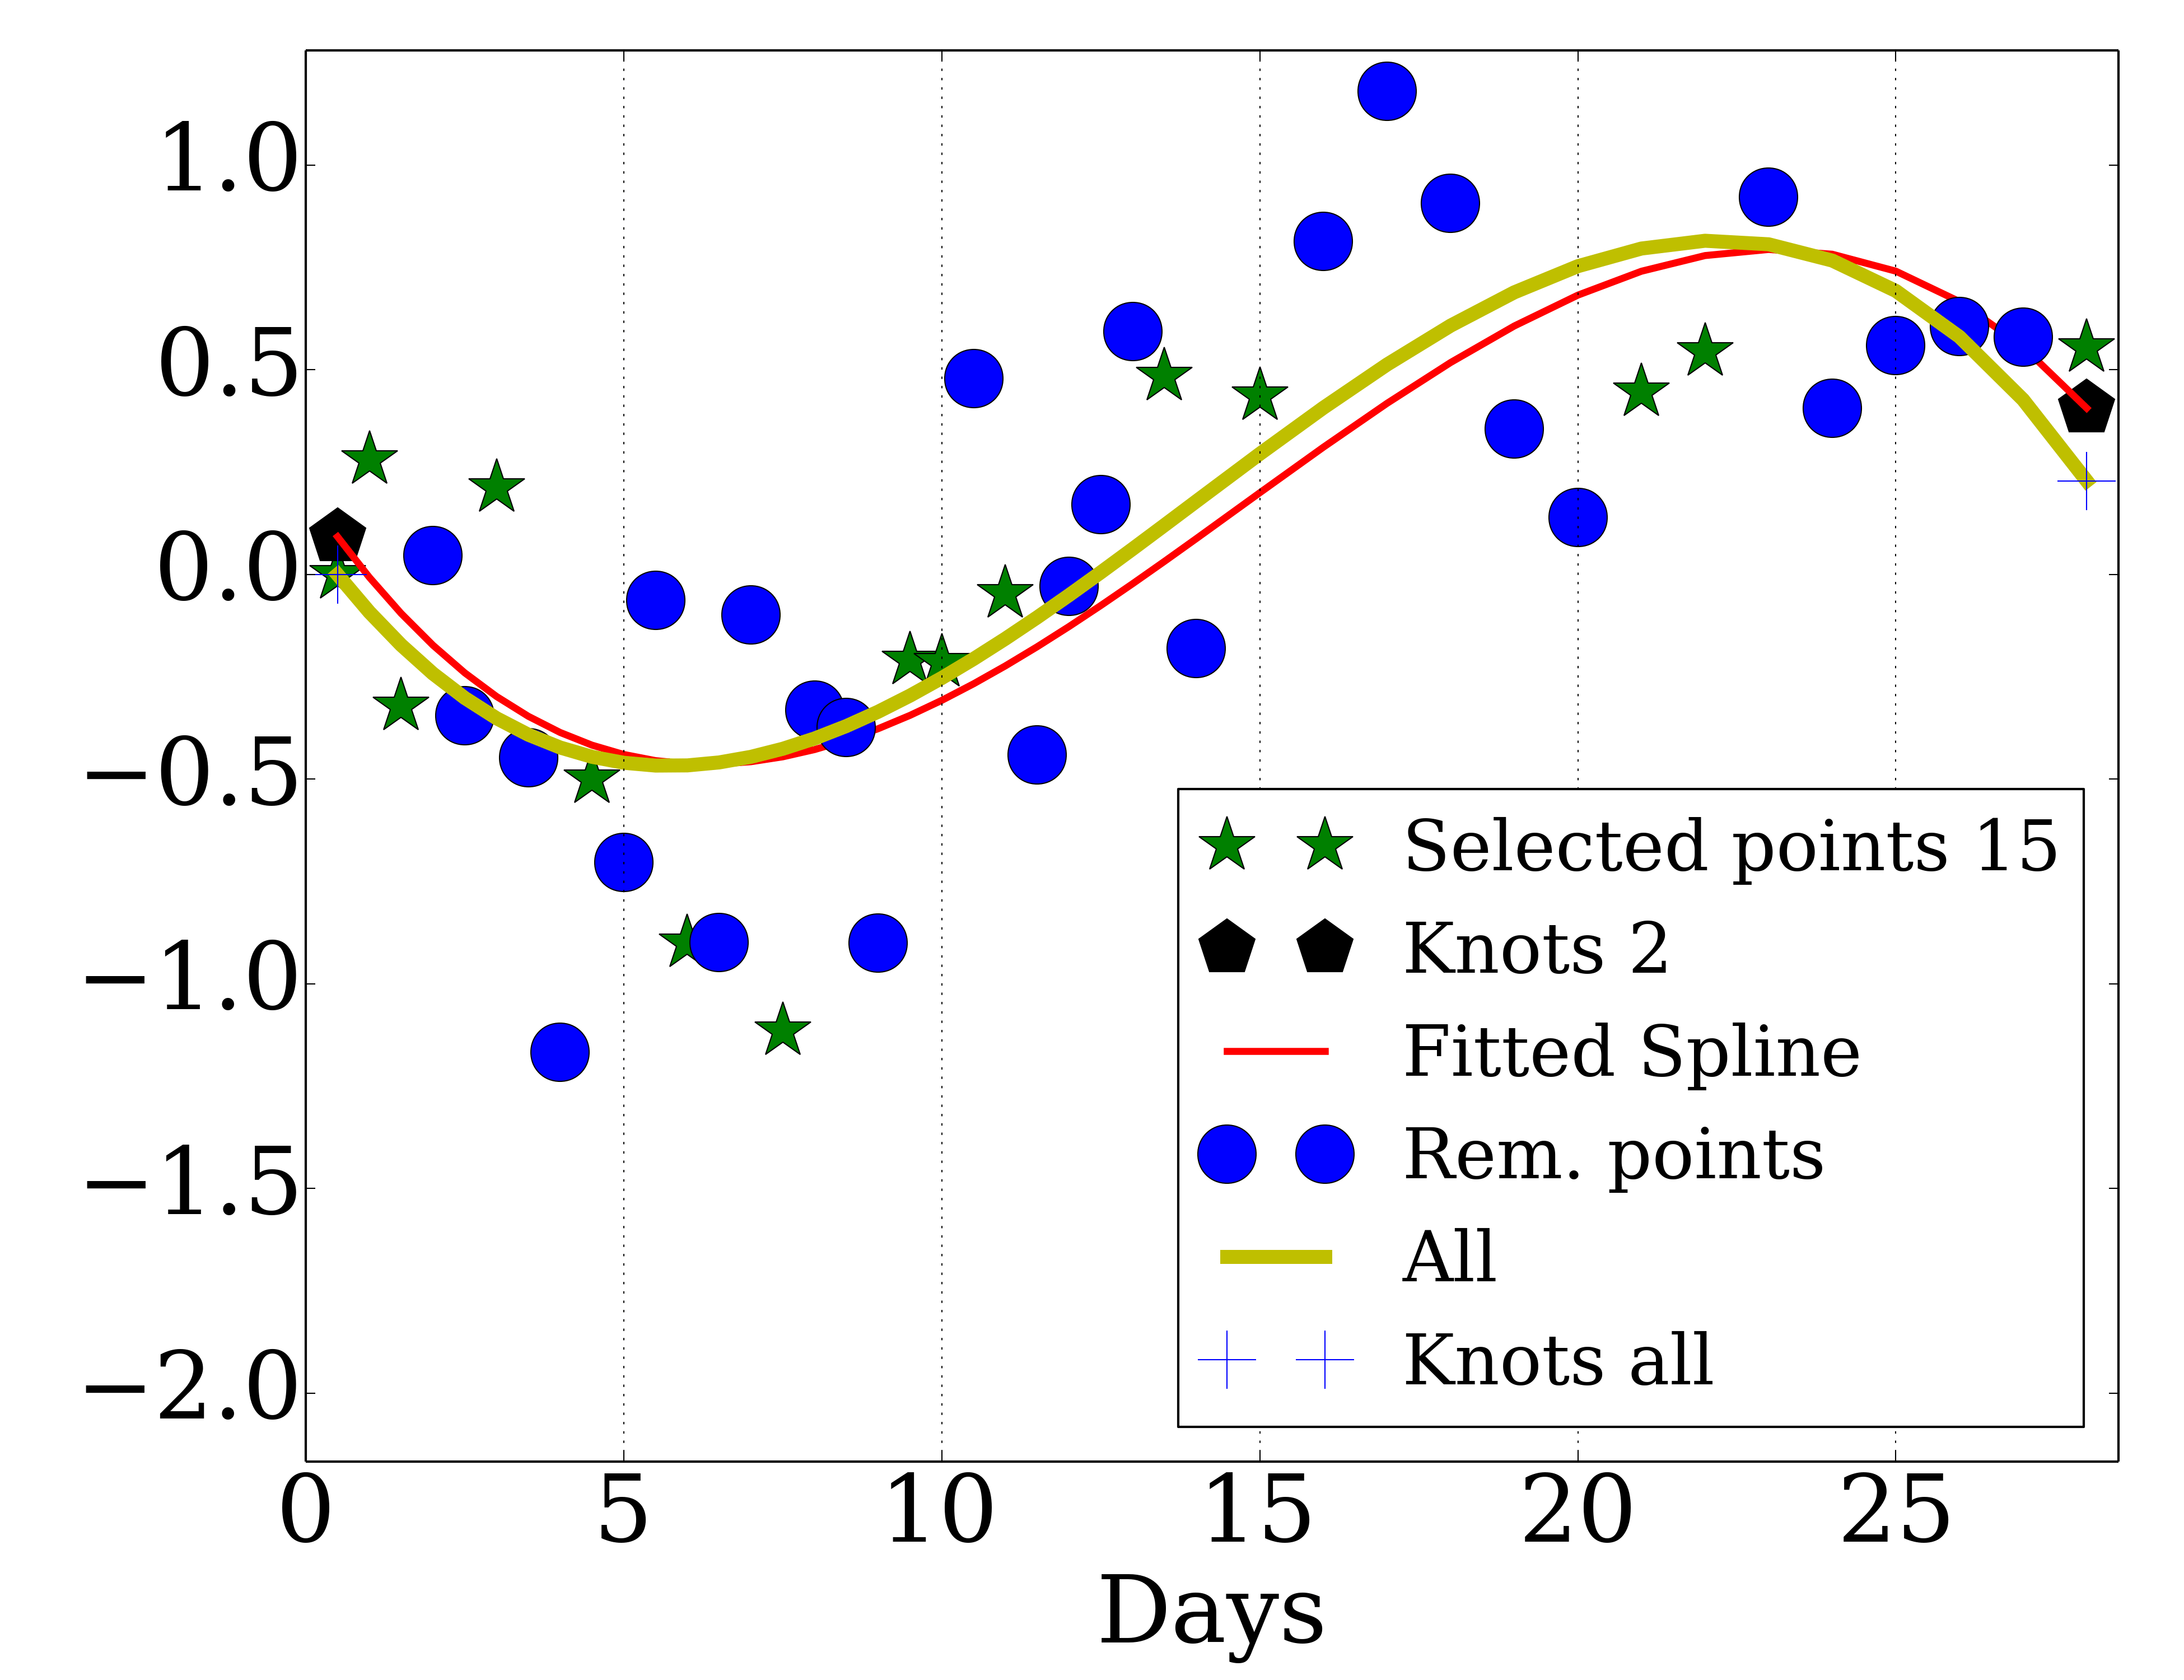
\includegraphics[scale=0.12]{{plots/newdata/splineplots15/ERB_15_all}.png}}
\hfill
\subfloat[NME3]{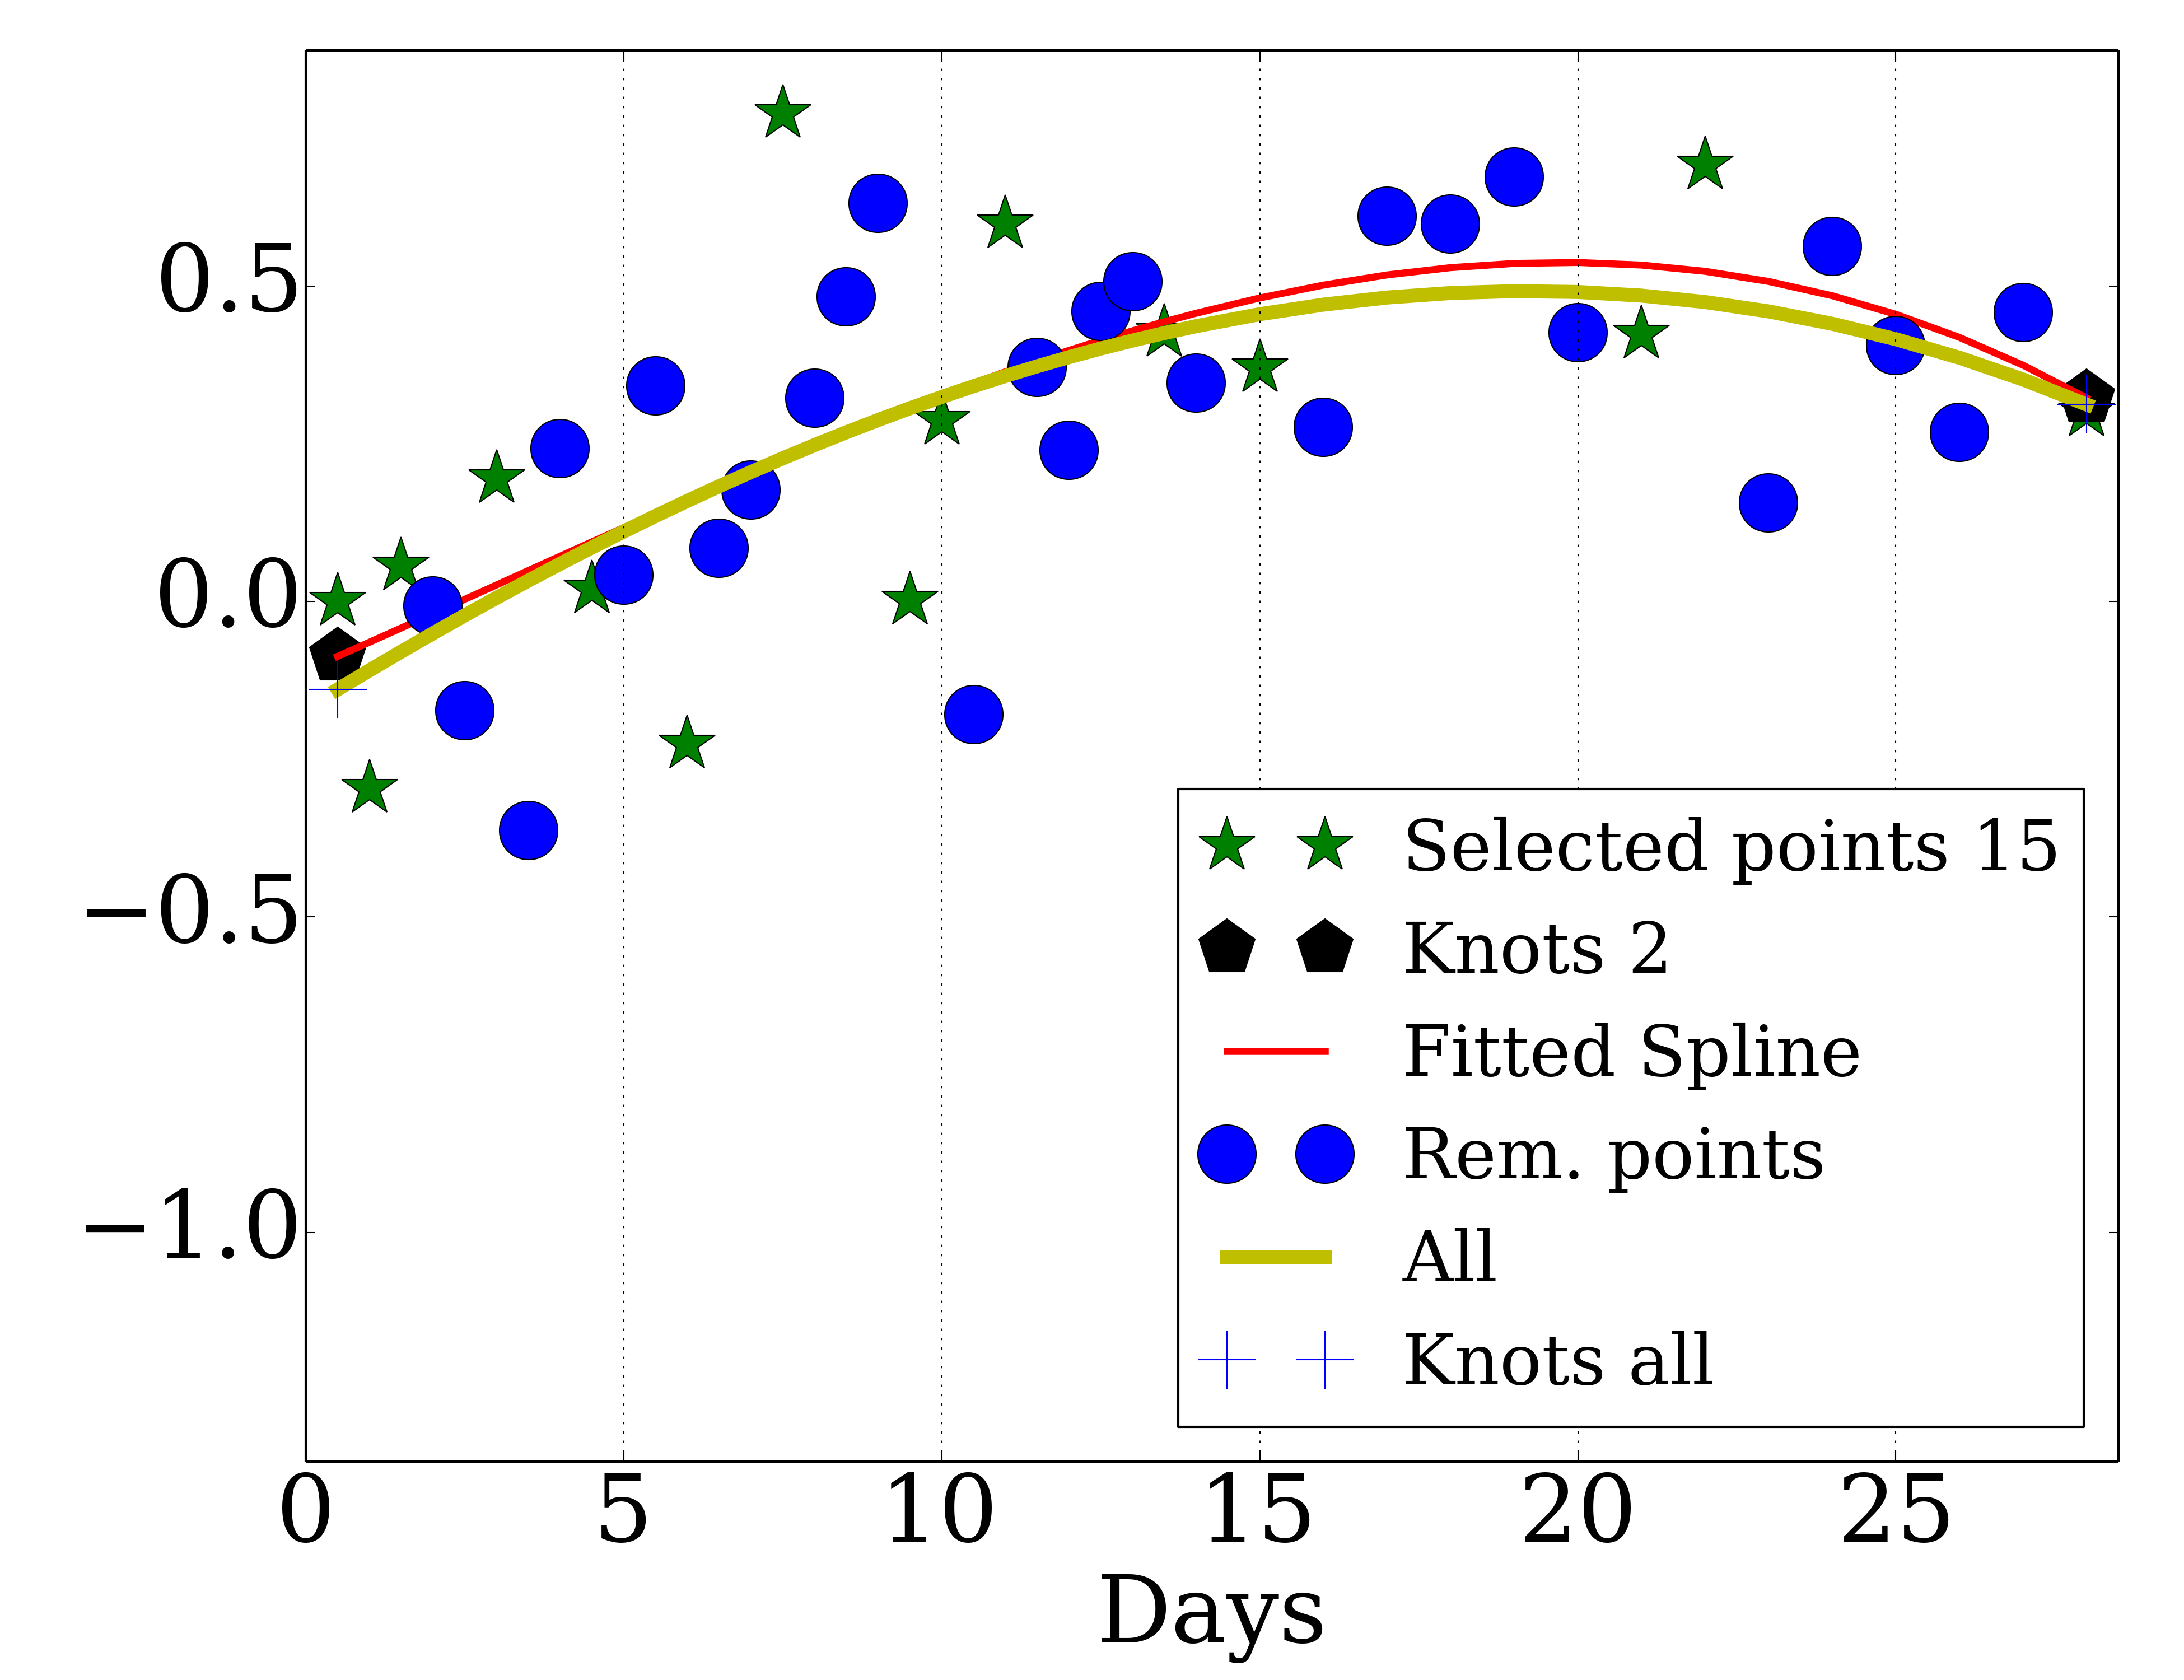
\includegraphics[scale=0.12]{{plots/newdata/splineplots15/NME3_15_all}.png}}
\hfill
\subfloat[POL2RA]{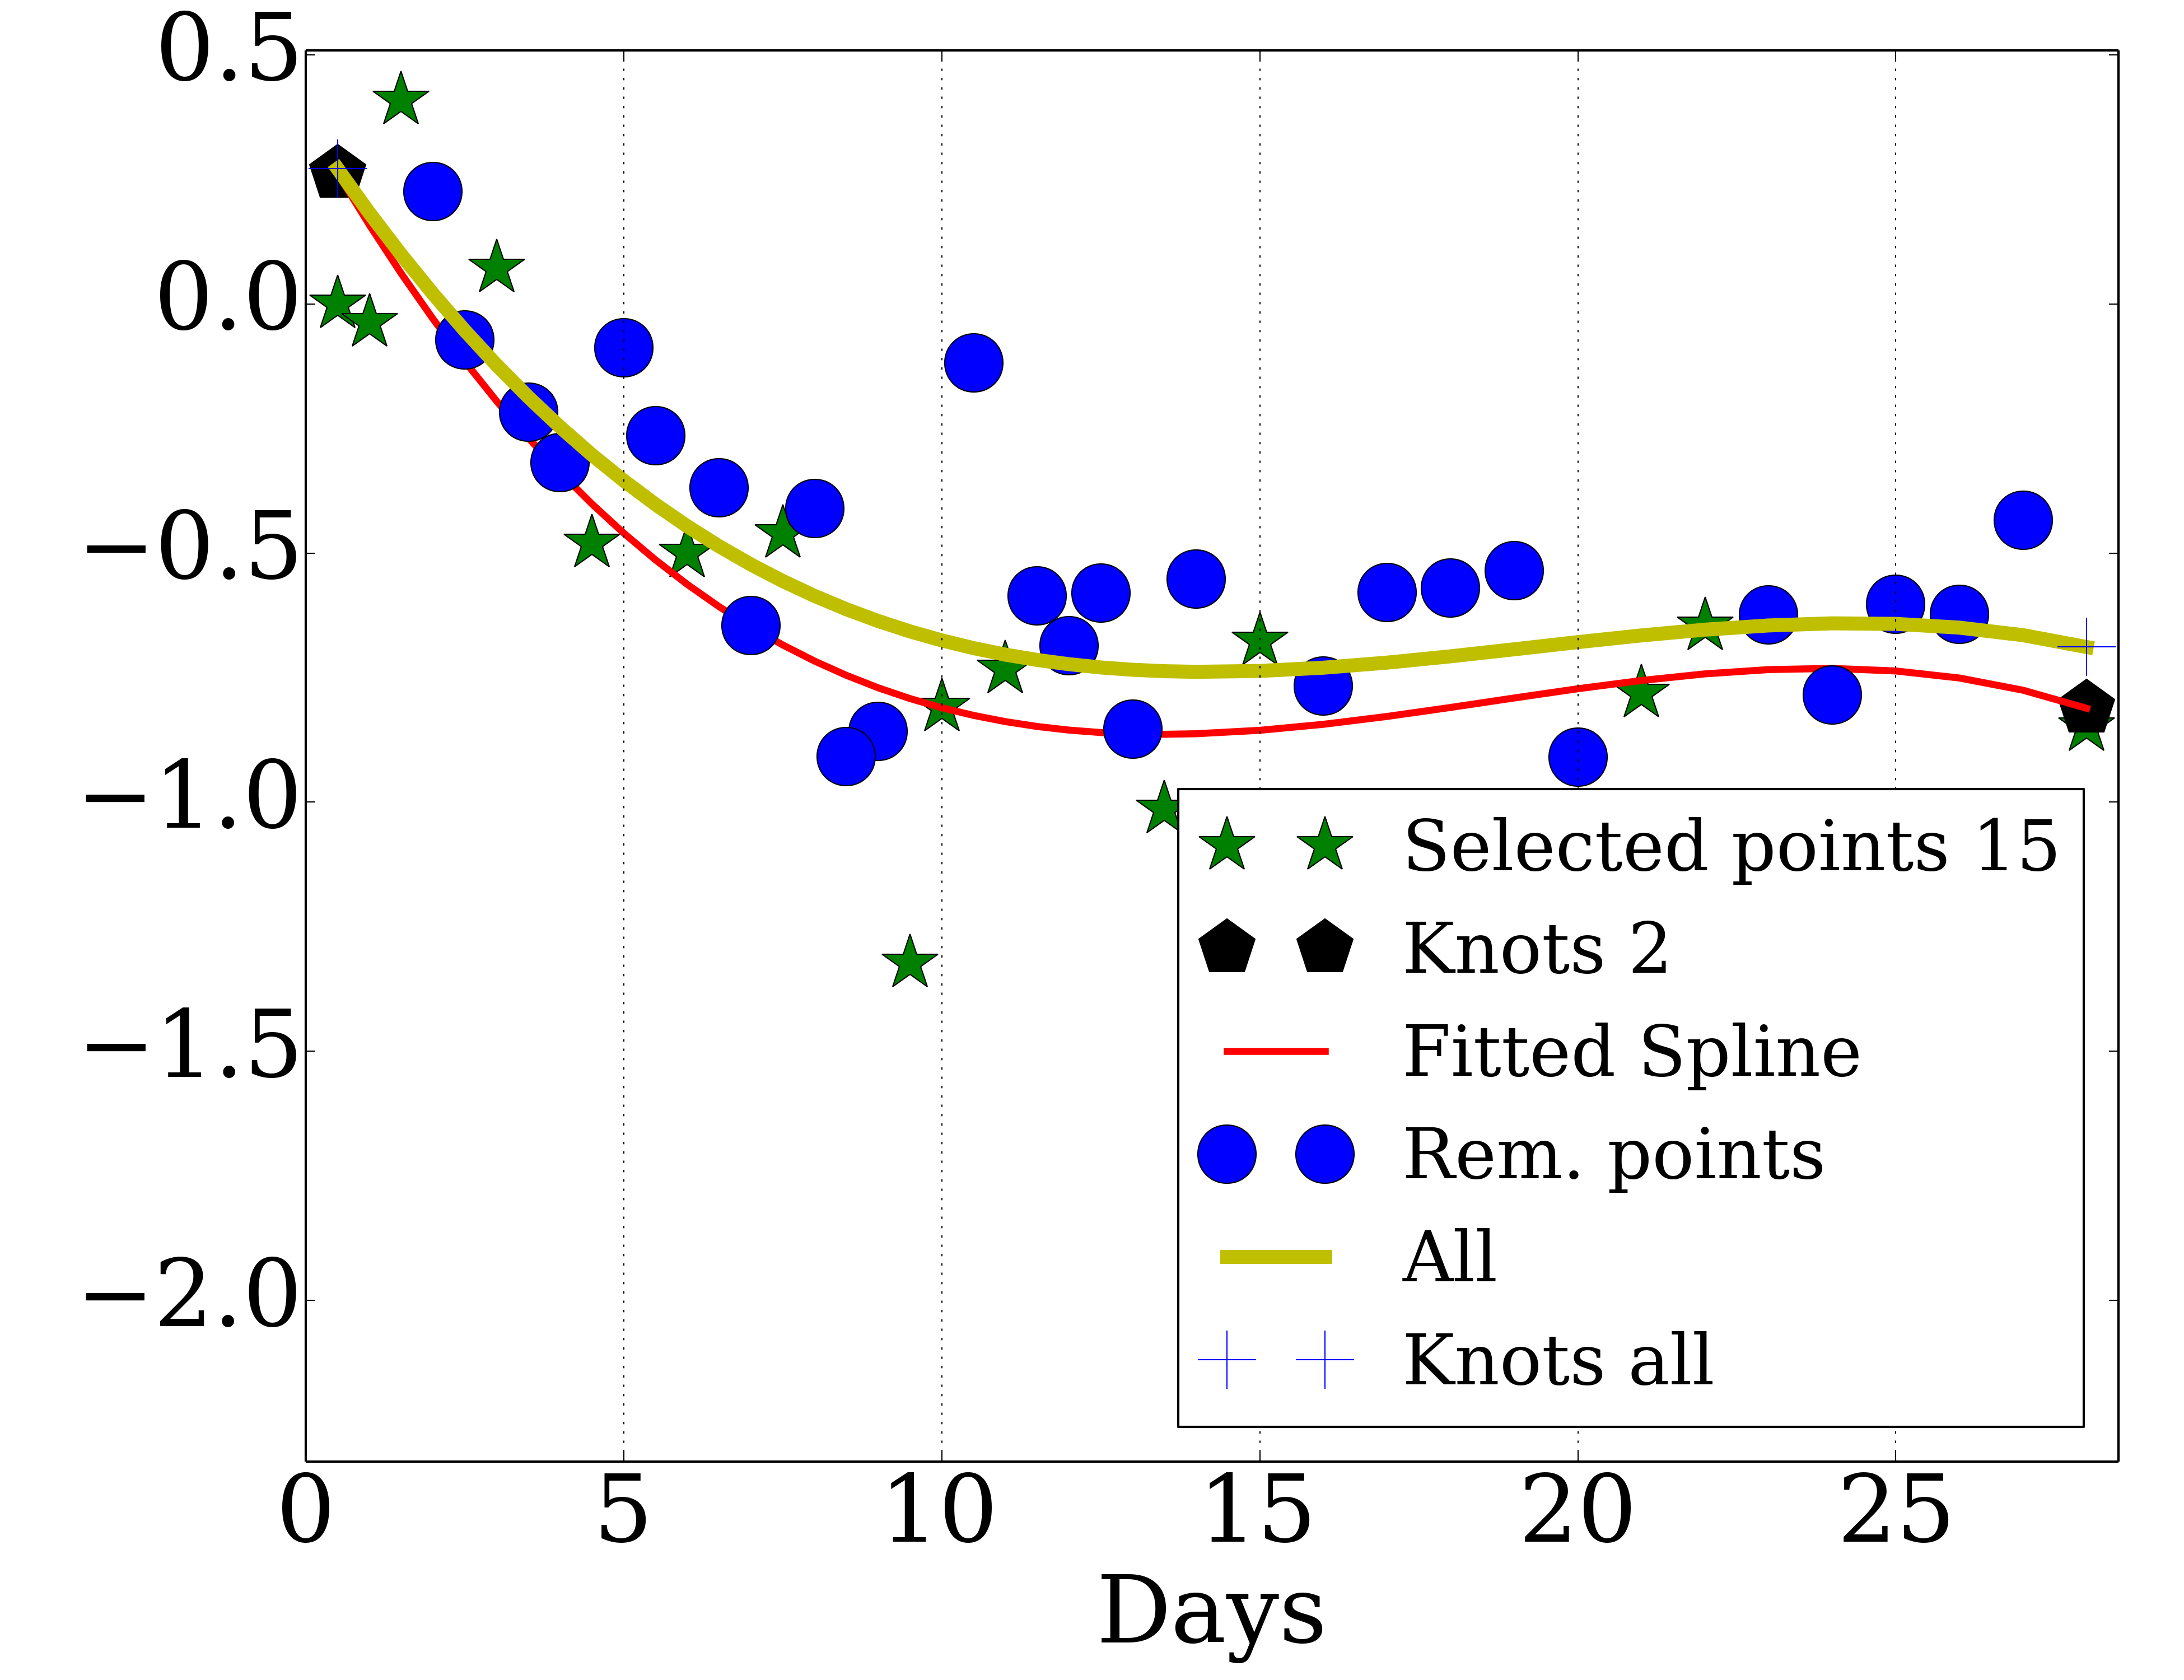
\includegraphics[scale=0.12]{{plots/newdata/splineplots15/polr2a_15_all}.png}}
\hfill
\end{minipage}
\caption{Expression profiles over several genes a) ERB, b) NME3, c) POL2RA}
\label{fig:sup3}
\end{figure}

\begin{figure}
\begin{minipage}{1.0\textwidth}
\subfloat[PDGFRA]{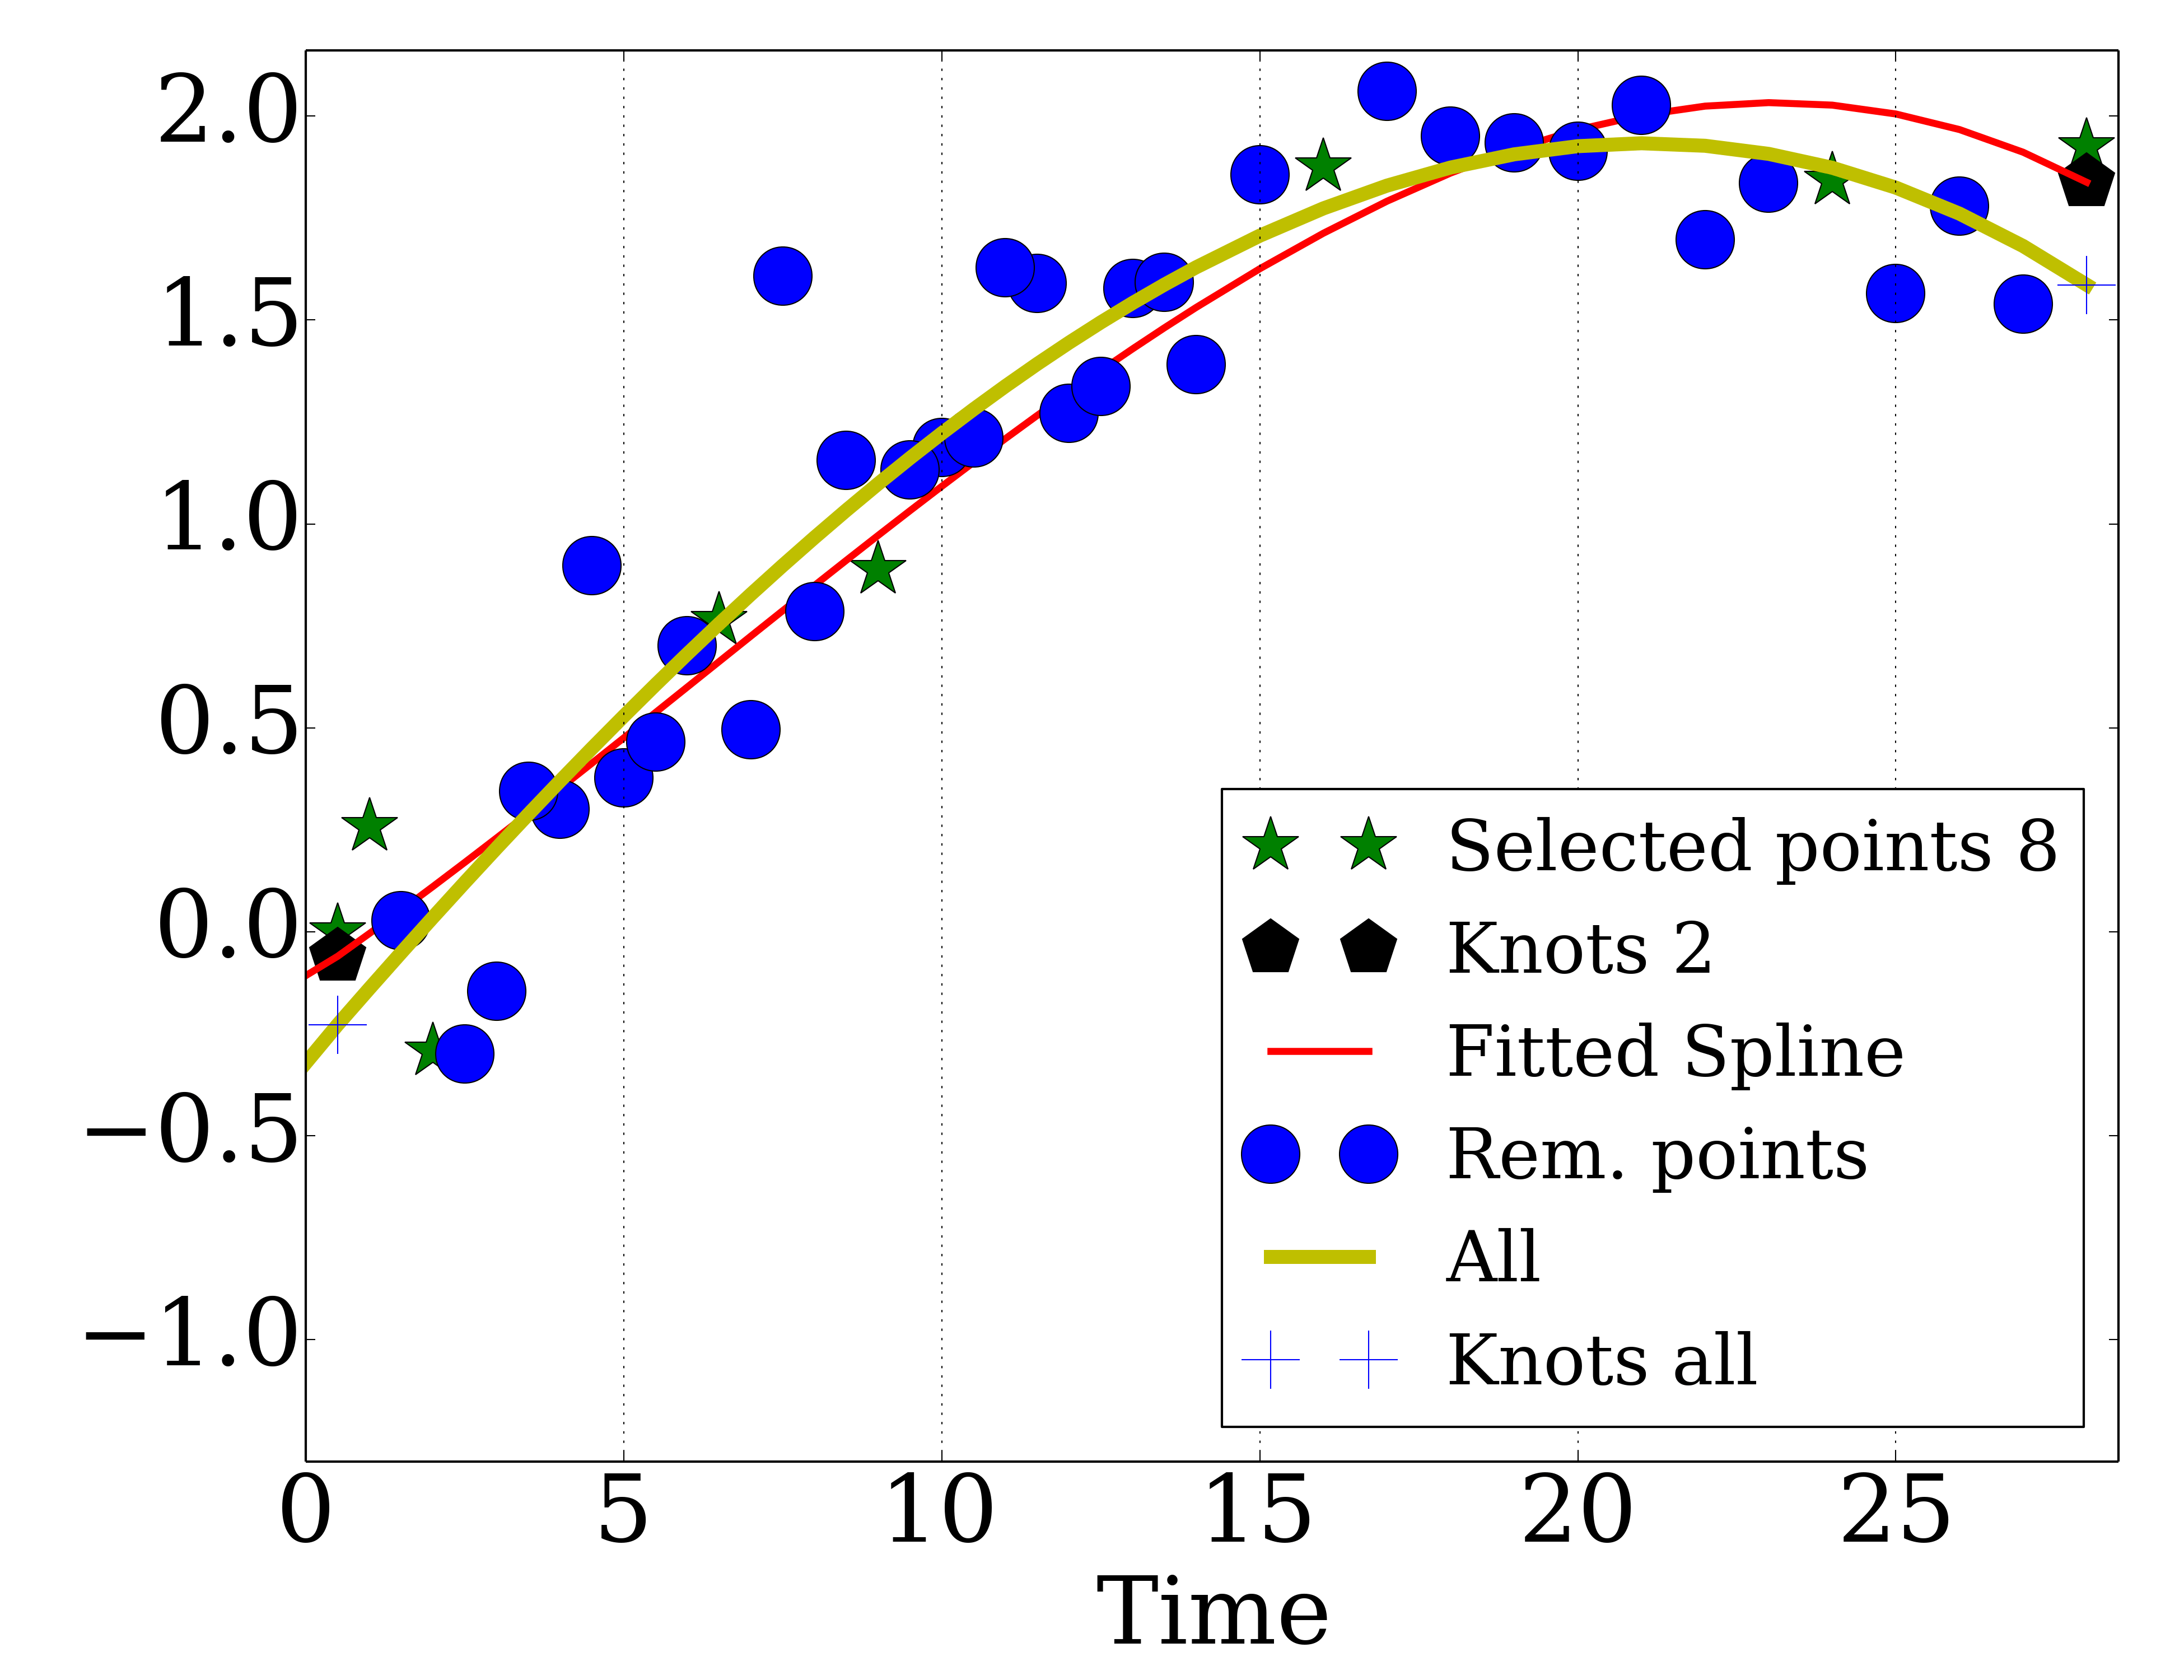
\includegraphics[scale=0.12]{{plots/newdata/splineplots8/PDGFRA_8_all}.png}}
\hfill
\subfloat[ELN]{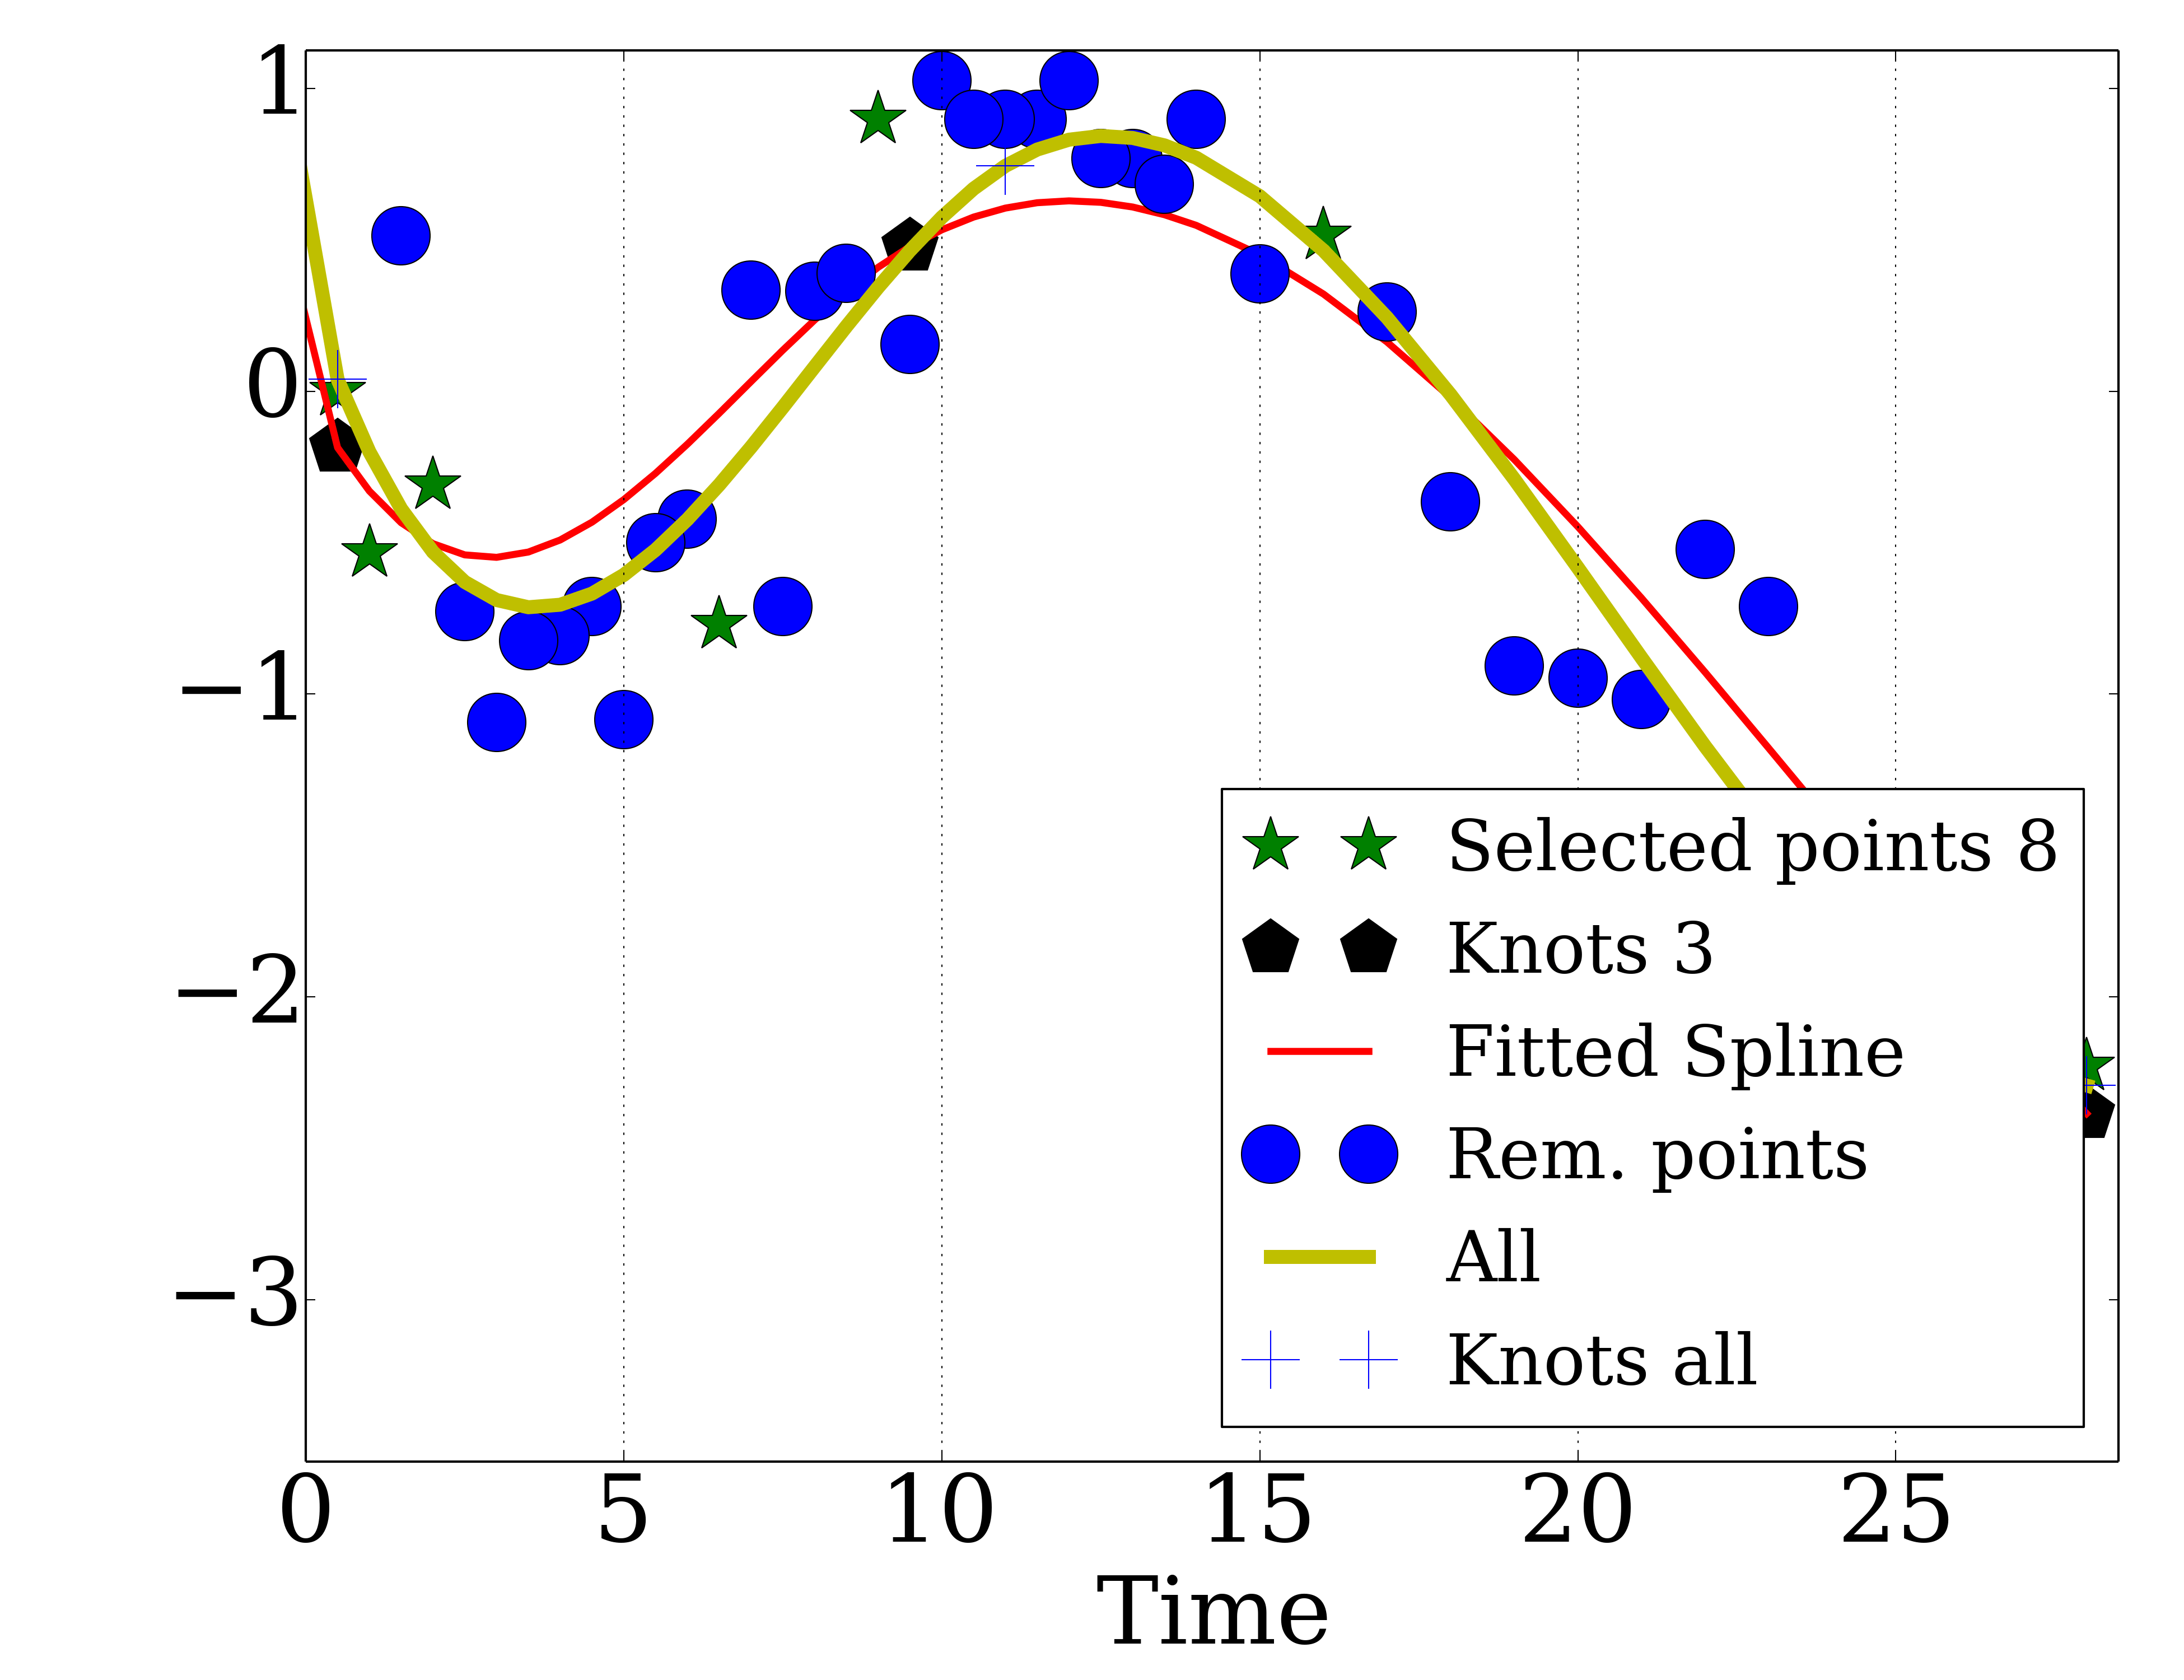
\includegraphics[scale=0.12]{{plots/newdata/splineplots8/Eln_8_all}.png}}
\hfill
\subfloat[INMT]{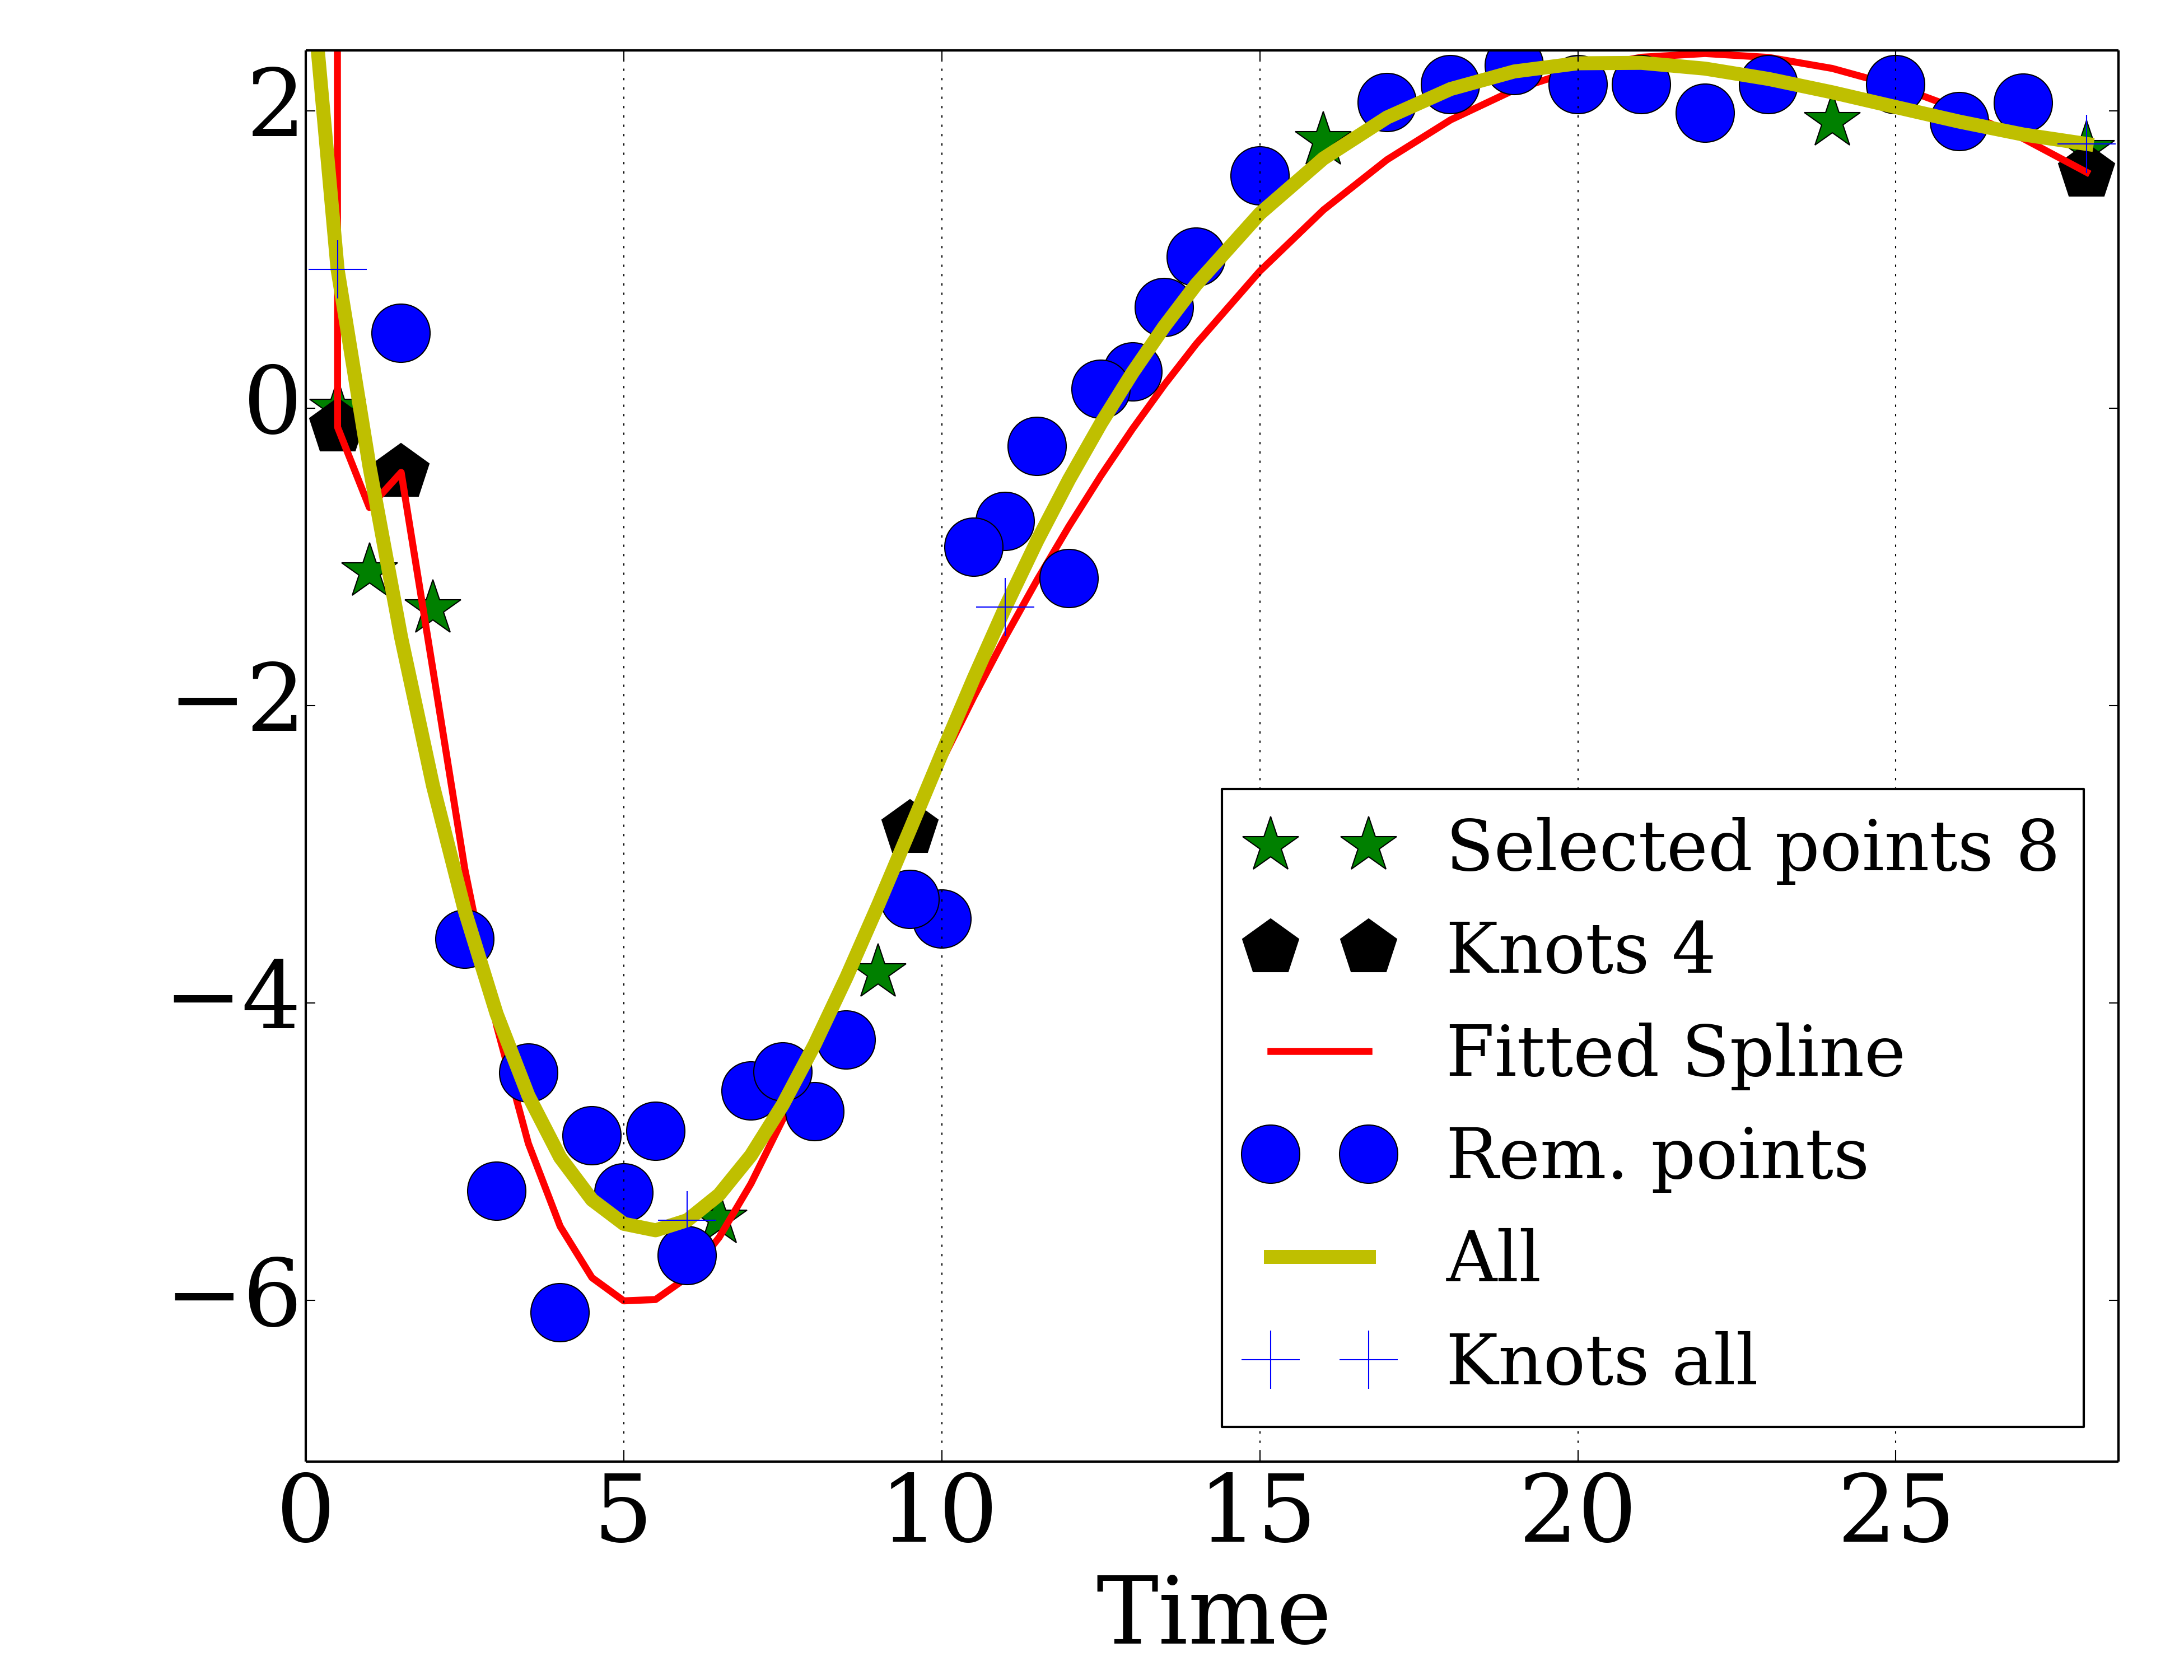
\includegraphics[scale=0.12]{{plots/newdata/splineplots8/INMT_8_all}.png}}
\hfill
\end{minipage}
\caption{Reconstructed expression profiles by $8$ points over genes a) PDGFRA, b) ELN, c) INMT}
\label{fig:sup4}
\end{figure}

\begin{figure}
\begin{minipage}{1.0\textwidth}
\subfloat[PDGFRA]{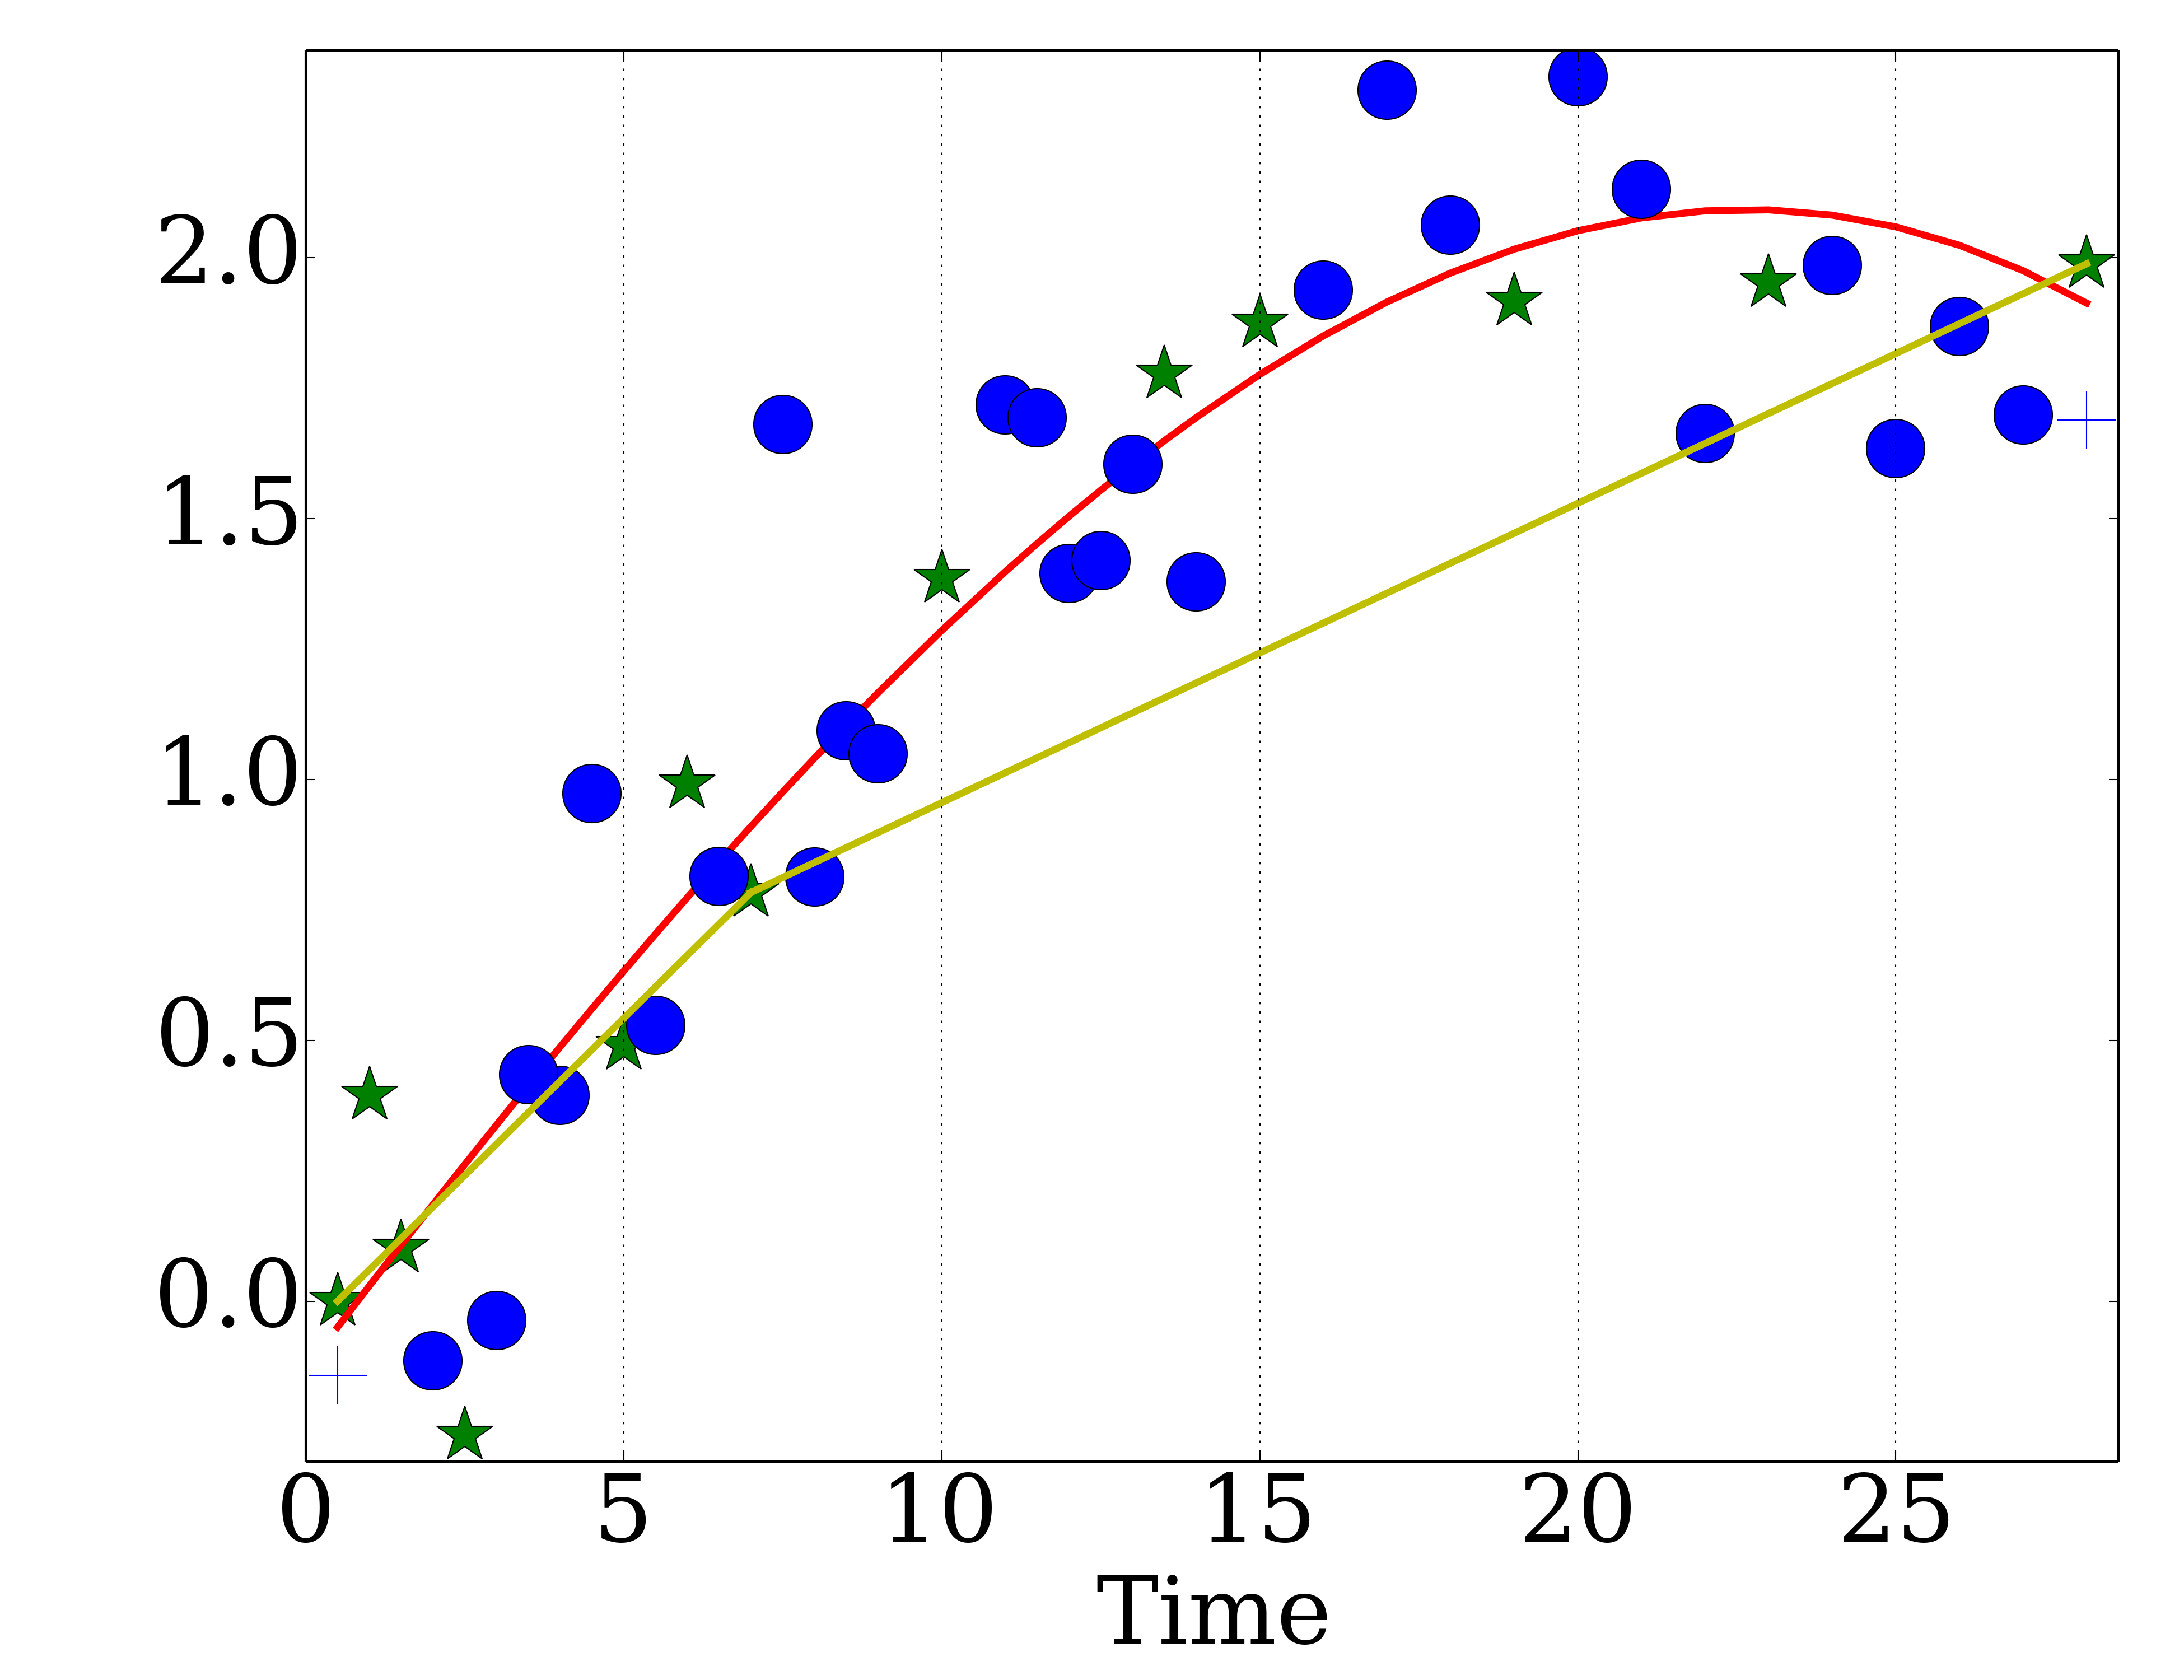
\includegraphics[scale=0.12]{{plots/newdata/splineAndLinear/17_PDGFRA_13_all}.png}}
\hfill
\subfloat[ELN]{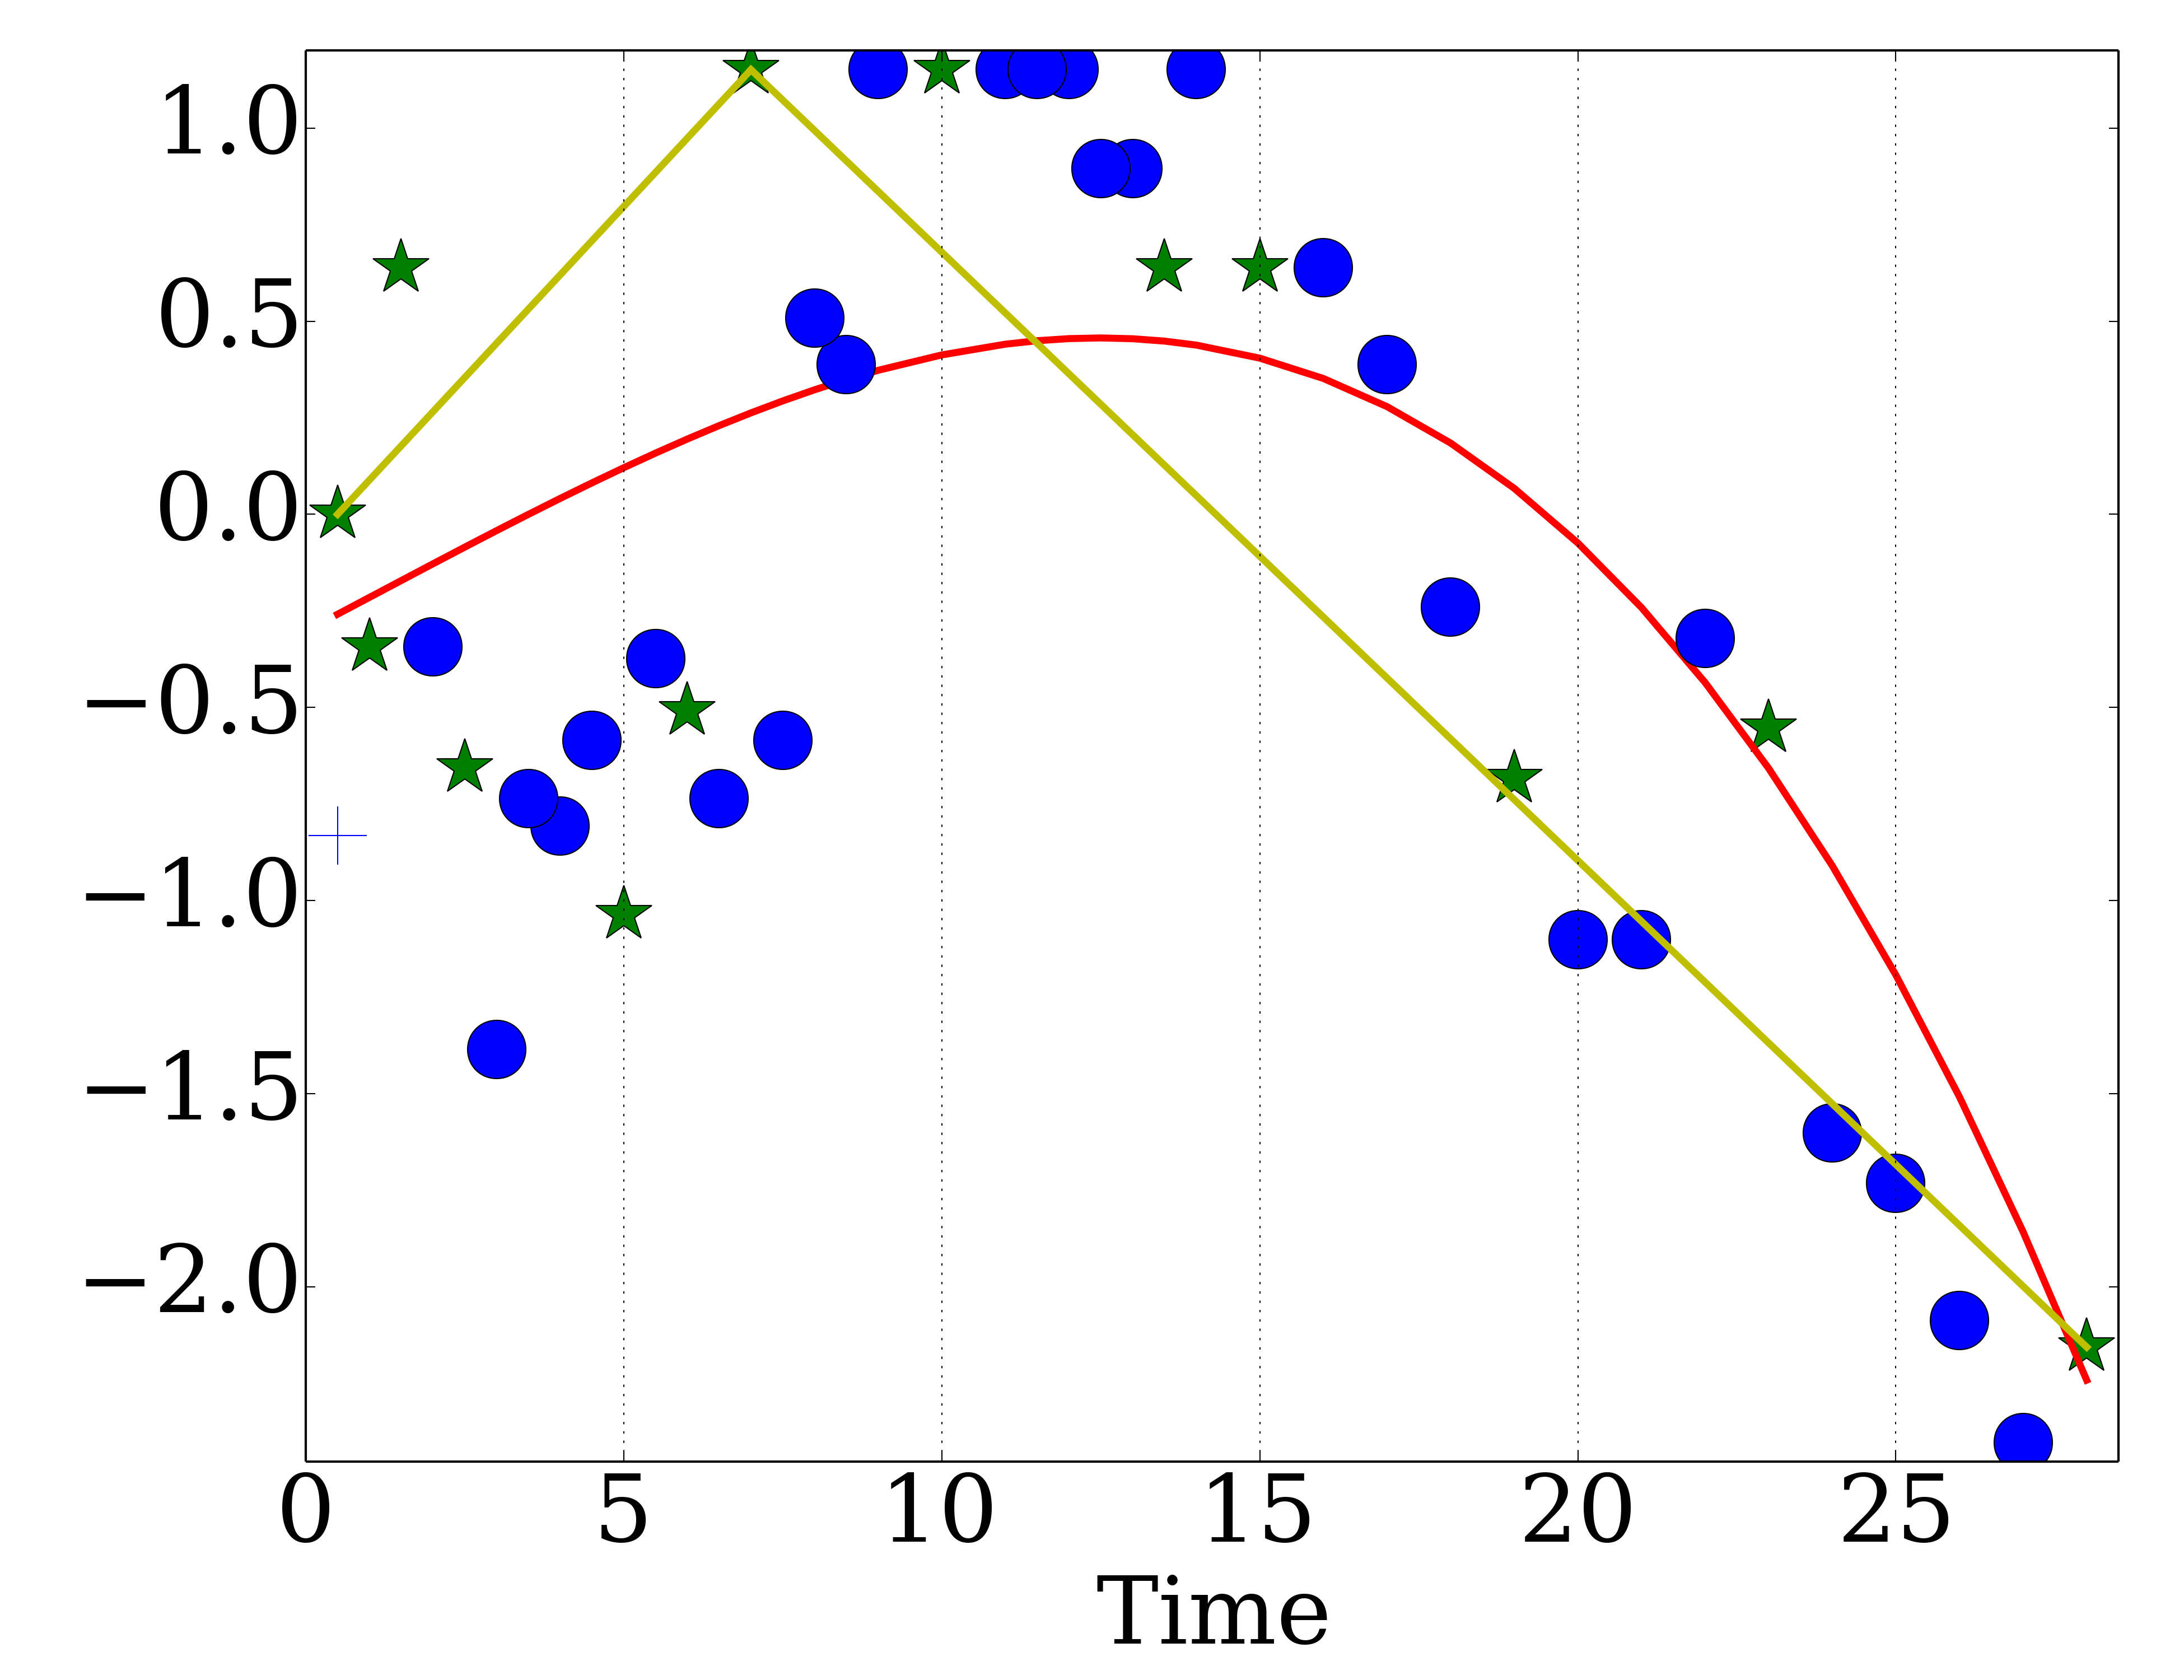
\includegraphics[scale=0.12]{{plots/newdata/splineAndLinear/14_Eln_13_all}.png}}
\hfill
\subfloat[LRAT]{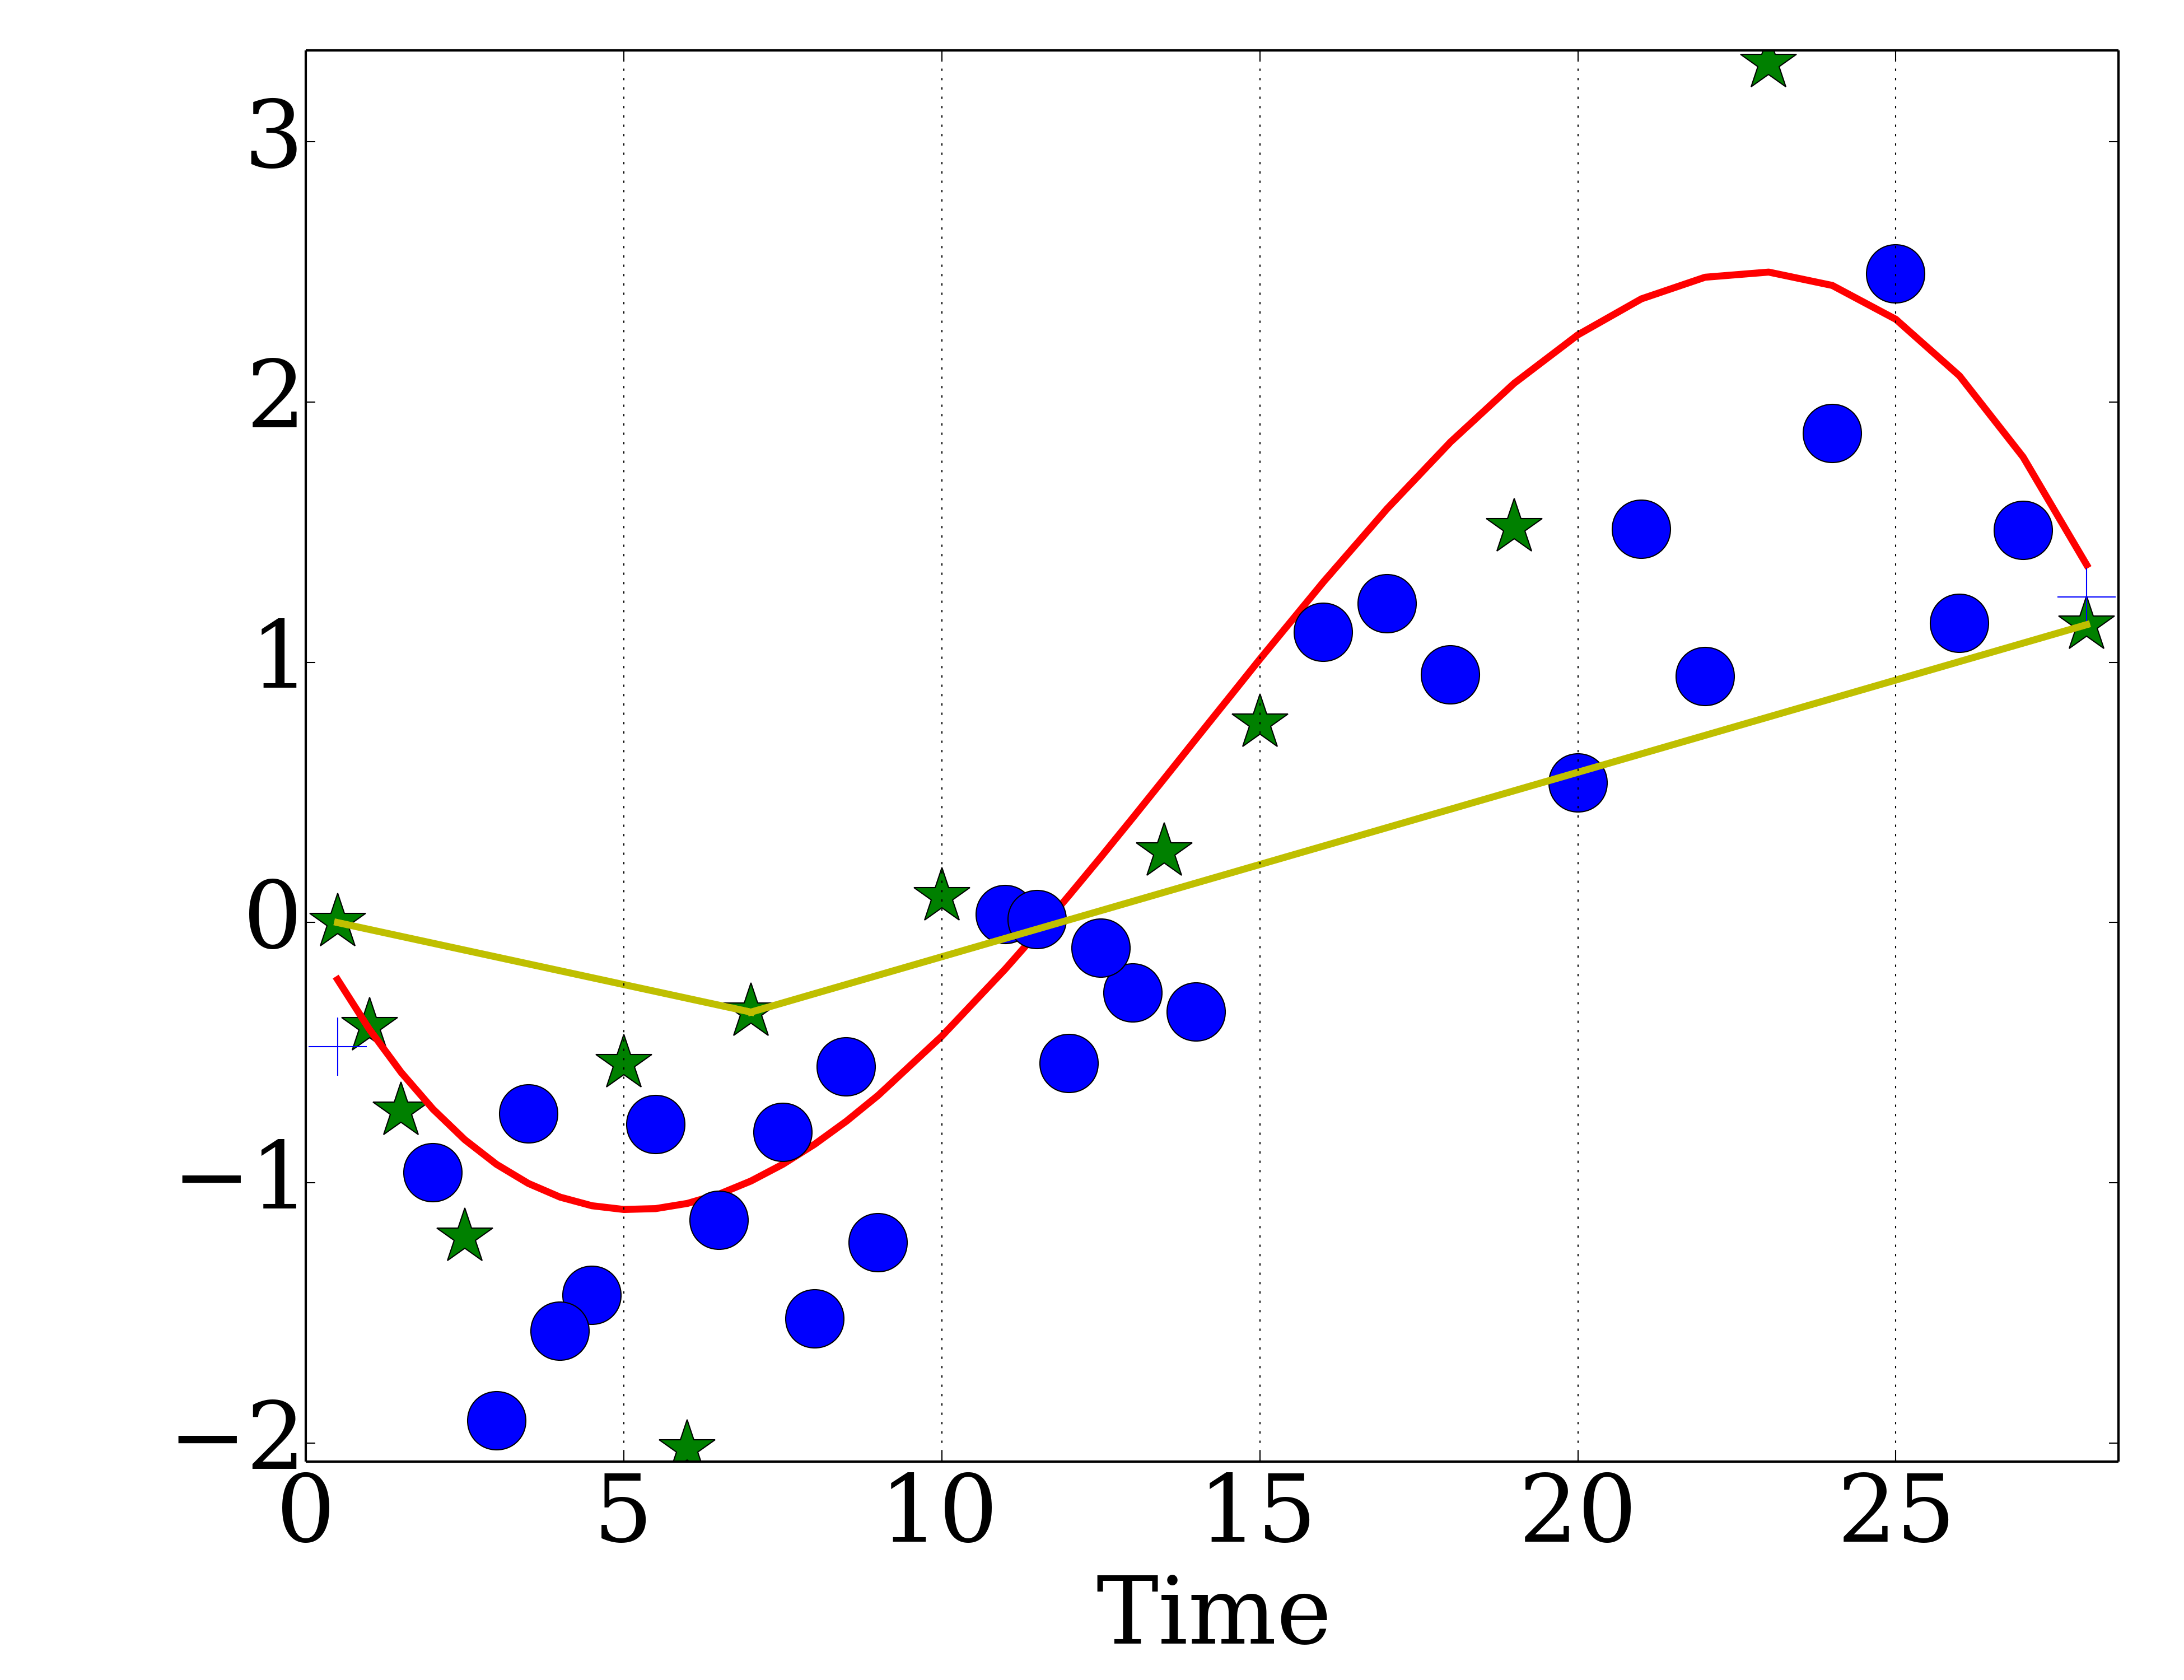
\includegraphics[scale=0.12]{{plots/newdata/splineAndLinear/1_LRAT_13_all}.png}}
\hfill
\end{minipage}
\caption{Comparison of \Tempselect and piecewise linear fitting over
  genes a) PDGFRA, b) ELN, c) LRAT}
\label{fig:sup5}
\end{figure}

\begin{figure}
\centering
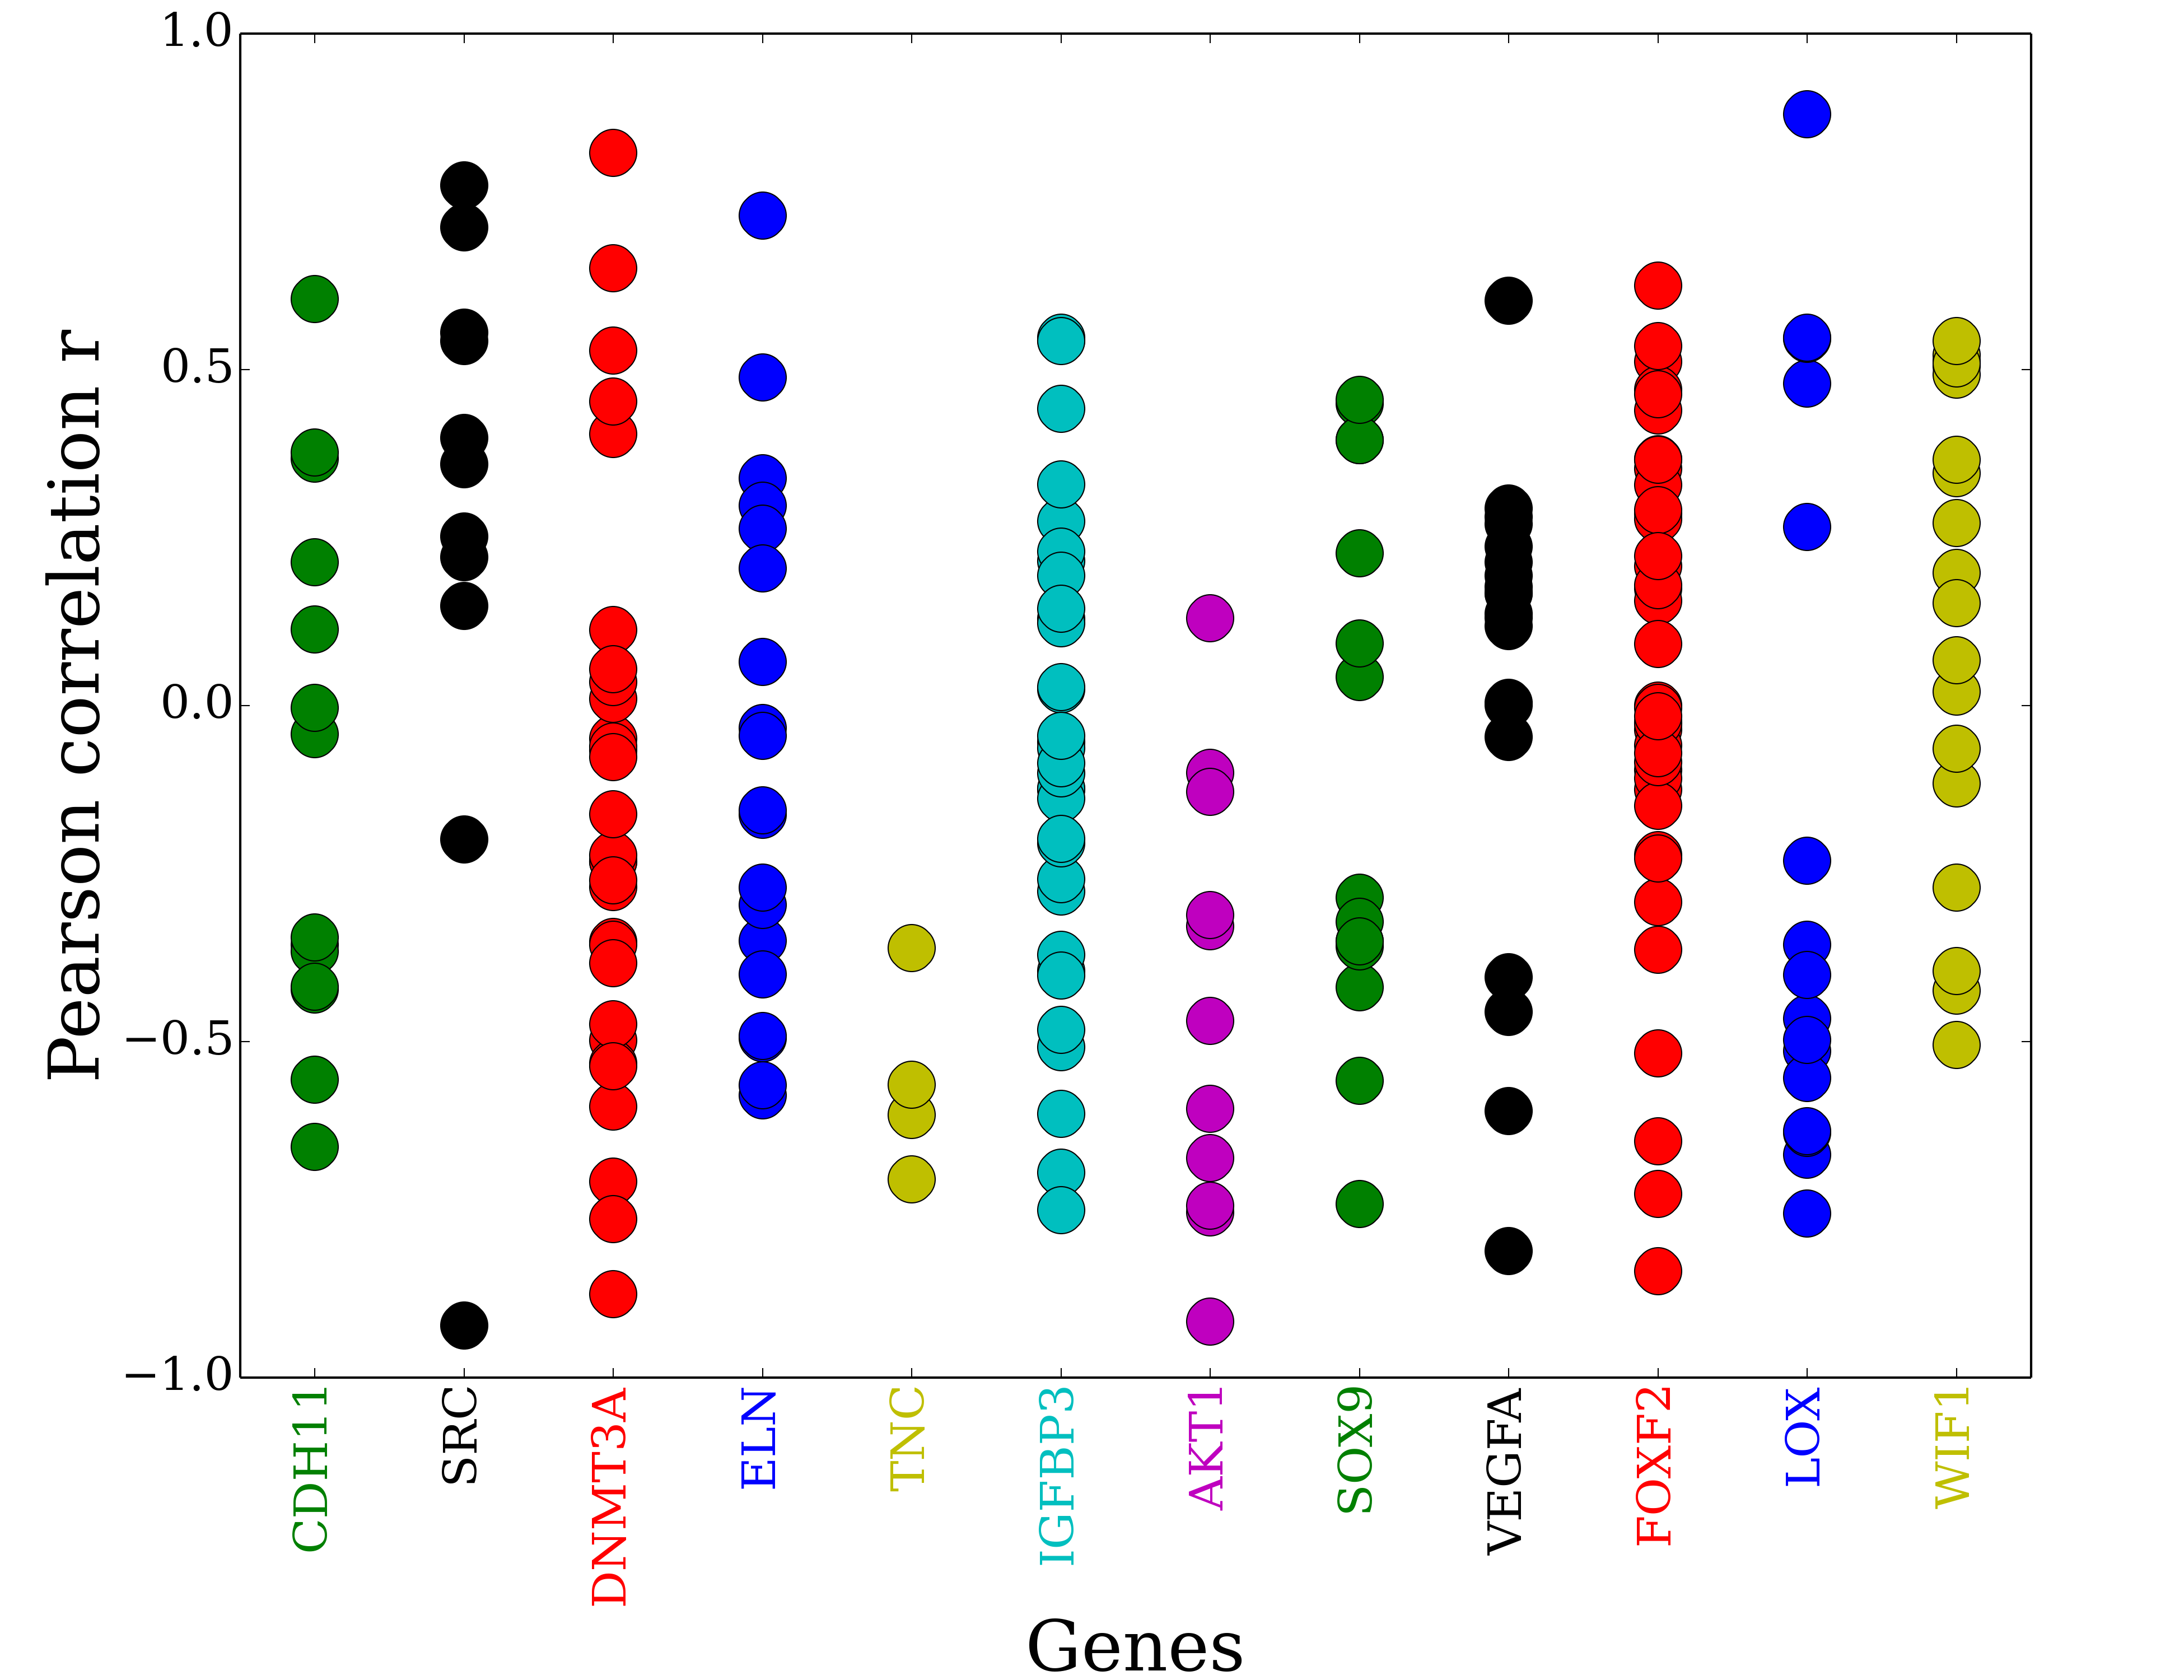
\includegraphics[scale=0.25]{{plots/meth/jointfigures_best/abs/valdist}.png}
\caption{Distribution of gene expression correlation for loci of each gene}
\label{fig:sup6}
\end{figure}


\section{Supplementary Tables}

\begin{table}[ht]
\centering
\begin{tabular}{|c|c|c|c|c|}
\hline
Gene & Number of loci  & & Gene & Number of loci  \\
\hline
Cdh11 & 14 & & Zfp536 & 16 \\
\hline
Src & 11 & & Igfbp3 & 34 \\
\hline
Sox9 & 16 & & Wif1 & 21 \\
\hline
Dnmt3a & 41 & & Vegfa & 20 \\
\hline
Eln & 20 & & Tnc & 4 \\
\hline
Foxf2 & 41 & & Lox & 17 \\
\hline
Akt1 & 11 & & &  \\
\hline
\end{tabular}
\caption{Summary of methylation dataset}
\label{tab:sup1}
\end{table}


% \begin{table}
% \centering
% \begin{tabular}{|c|c|c|c|c|}
% \hline
% Gene & $r$  & & Gene & $r$ \\
% \hline
% Cdh11 & $0.60$ & & Lox & $0.88$ \\
% \hline
% Src & $0.77$ & & Igfbp3 & $0.55$ \\
% \hline
% Sox9 & $0.45$ & & Wif1 & $0.54$ \\
% \hline
% Dnmt3a & $0.82$ & & Vegfa & $0.60$ \\
% \hline
% Eln & $0.72$ & & Tnc & $-0.36$ \\
% \hline
% Foxf2 & $0.62$ & & & \\
% \hline
% Akt1 & $0.13$ & & &  \\
% \hline
% \end{tabular}
% \caption{Pearson correlation $r$  between expression and
%   methylation datasets over $8$ time points for each gene.}
% \label{tab:sup2}
% \end{table}

\begin{table}
\centering
\begin{tabular}{|c|c|c|c|c|}
\hline
Gene & $r$  & & Gene & $r$ \\
\hline
Cdh11 & $-0.65$ & & Lox & $0.88$ \\
\hline
Src & $-0.92$ & & Igfbp3 & $-0.75$ \\
\hline
Sox9 & $-0.74$ & & Wif1 & $0.54$ \\
\hline
Dnmt3a & $-0.876$ & & Vegfa & $-0.81$ \\
\hline
Eln & $0.72$ & & Tnc & $-0.70$ \\
\hline
Foxf2 & $-0.84$ & & & \\
\hline
Akt1 & $-0.91$ & & &  \\
\hline
\end{tabular}
\caption{Pearson correlation $r$  between expression and
  methylation datasets over $8$ time points for each gene.}
\label{tab:sup2}
\end{table}

\newpage

\bibliographystyle{plain}
\bibliography{expressbib}

\end{document}
